%% Enunturi Electricitate si Magnetism %%

\section*{3. ELECTRICITATE Şi MAGNETISM*}

% Problemele notate cu * conțin noțiuni care nu sunt cuprinse în programa analitică a examenului de admitere din acest an, dar sunt utile pentru pregătirea candidaților.

3.1. Două generatoare de tensiune electromotoare de $7 \mathrm{~V}$ și de rezistență interioară de $0,2 \Omega$ sunt legate în serie la bornele unui rezistor de rezistență de $6,6 \Omega$. Căldura disipată de rezistența de $6,6 \Omega$ în timp de un minut este:\\ A) $1584 \mathrm{~J}$; B) $1600 \mathrm{~J}$; C) $1580 \mathrm{~J}$; D) $1800 \mathrm{~J}$; E) $2050 \mathrm{~J}$; F) $3000 \mathrm{~J}$.\\ (Ion M. Popescu)\\

3.2. Un conductor de cupru ( $\rho_{\mathrm{Cu}}=1,7 \cdot 10^{-8} \Omega \mathrm{~m}$ ) lung de $160 \mathrm{~m}$ şi cu secțiunea de $16 \mathrm{~mm}^{2}$ este conectat la tensiunea de $170 \mathrm{~V}$. De-a lungul conductorului producându-se o cădere de tensiune de $6 \%$, prin conductor trece un curent electric de intensitate:\\ A) $55 \mathrm{~A}$; B) $65 \mathrm{~A}$; C) $40 \mathrm{~A}$; D) $100 \mathrm{~A}$; E) $60 \mathrm{~A}$; F) $75 \mathrm{~A}$.\\ (Ion M. Popescu)\\

3.3. În rețeaua din Fig. 3.1 se dau: $E=5,5 \mathrm{~V}, \quad R_{1}=1 \Omega, \quad R_{2}=2 \Omega, \quad R_{3}=3 \Omega$. Schimbând locul sursei $E$ cu cel al ampermetrului A , acesta indică:\\ A) $1 \mathrm{~A}$; B) $0,8 \mathrm{~A}$; C) $5 \mathrm{~A}$; D) $0,5 \mathrm{~A}$; E) $0,8 \mathrm{~A}$; F) $2 \mathrm{~A}$.\\ (Ion M. Popescu)\\ 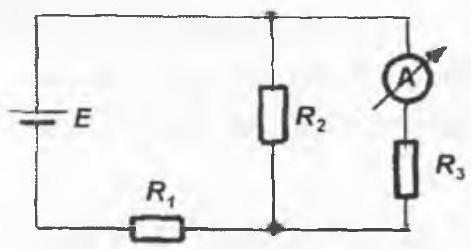
\includegraphics[max width=\textwidth, center]{2025_07_01_5b3ff9fa0d508c8e9f17g-144} Fig. 3.1\\

3.4. Dacă două generatoare electrice cu tensiunea electromotoare de $8 \mathrm{~V}$ şi rezistența interioară de $0,2 \Omega$ sunt legate în serie la bornele unui rezistor cu rezistența de $7,6 \Omega$, prin fiecare generator electric trece curentul electric de intensitate:\\ A) $1,5 \mathrm{~A}$; B) $2 \mathrm{~A}$; C) $1,8 \mathrm{~A}$; D) $2,5 \mathrm{~A}$; E) $3 \mathrm{~A}$; F) $0,5 \mathrm{~A}$.\\ (Ion M. Popescu)\\

3.5. Dacă două generatoare electrice cu tensiunea electromotoare de $10 \mathrm{~V}$ și rezistența interioară de $0,2 \Omega$ sunt legate în paralel la bornele unui rezistor cu rezistența de $9,9 \Omega$, prin fiecare generator electric trece curentul electric de intensitate:\\ A) $0,6 \mathrm{~A}$; B) $0,4 \mathrm{~A}$; C) $0,5 \mathrm{~A}$; D) $1 \mathrm{~A}$; E) $3 \mathrm{~A}$; F) $2 \mathrm{~A}$.\\ (Ion M. Popescu)\\

3.6. Un generator electric care produce într-o rezistență de $16 \Omega$ aceeași putere electrică ca într-o rezistență de $25 \Omega$, are rezistența interioară egală cu:\\ A) $16 \Omega$; B) $22 \Omega$; C) $10 \Omega$; D) $20 \Omega$; E) $5 \Omega$; F) $30 \Omega$.\\ (Ion M. Popescu)\\

3.7. Un încălzitor are două rezistoare $R_{\mathrm{J}}$ şi $R_{2}$. Timpul de fierbere a unei mase de apă cu încălzitorul este $t_{1}=20 \mathrm{~s}$, dacă se conectează numai primul rezistor şi $t_{2}=30 \mathrm{~s}$, dacă se conectează numai al doilea rezistor. Dacă se conectează ambele rezistoare în paralel, timpul de fierbere a apei este:\\ A) $30 \mathrm{~s}$; B) $20 \mathrm{~s}$; C) $25 \mathrm{~s}$; D) $4 \mathrm{~s}$; E) $16 \mathrm{~s}$; F) $12 \mathrm{~s}$.\\ (Ion M. Popescu)\\

3.8. Un bec şi un reostat sunt legate în serie şi formează un circuit electric, consumând împreună $200 \mathrm{~W}$. Tensiunea la bornele becului fiind $60 \mathrm{~V}$ şi rezistenţa reostatului $20 \Omega$, prin circuitul electric trece curentul electric de intensitate:\\ A) $12 \mathrm{~A}$; B) $5 \mathrm{~A}$; C) $1 \mathrm{~A}$; D) $3 \mathrm{~A}$; E) $2 \mathrm{~A}$; F) $2,5 \mathrm{~A}$.\\ (Ion M. Popescu)\\

3.9.* Un corp cu suprafața de $50 \mathrm{~cm}^{2}$ este legat la catodul unei băi de nichelare prin care trece un curent electric cu intensitatea de $1,0 \mathrm{~A}$. Pe suprafaţa corpului se depune un strat de nichel ( $\rho_{\mathrm{Ni}}=8,8 \cdot 10^{3} \mathrm{~kg} / \mathrm{m}^{3}, k_{\mathrm{Ni}}=0,203 \mathrm{~mg} / \mathrm{C}$ ) gros de $0,1015 \mathrm{~mm}$ în timpul de:\\ A) $22 \mathrm{~s}$; B) $40 \mathrm{~s}$; C) $20 \mathrm{~s}$; D) $32 \mathrm{~s}$; E) $15 \mathrm{~s}$; F) $100 \mathrm{~s}$.\\ (Ion M. Popescu)\\

3.10. Se consideră un circuit format dintr-un rezistor legat la o sursă cu tensiune electromotoare de $2 \mathrm{~V}$ şi rezistența interioară $r=1 \Omega$. Căderea de tensiune pe rezistența interioară a sursei, ştiind că puterea disipată pe rezistor este maximă, va fi:\\ A) $5 \mathrm{~V}$; B) $0,1 \mathrm{~V}$; C) $1 \mathrm{~V}$; D) $3 \mathrm{~V}$; E) $0,2 \mathrm{~V}$; F) $1,5 \mathrm{~V}$.\\ (Niculae Puşcaş)\\

3.11. Se consideră trei rezistoare: $R_{1}=R ; R_{2}=R+R_{0} ; R_{3}=R-R_{0}$. Valorile rezistențelor astfel ca la legarea în serie a acestora rezistența echivalentă să fie $9 \Omega$, iar la legarea în paralel să fie $12 / 13 \Omega$, sunt:\\ A) $3 \Omega , 4 \Omega , 2 \Omega$; B) $10 \Omega , 1,5 \Omega , 2 \Omega$; C) $1 \Omega , 5 \Omega , 3 \Omega$; D) $1 \Omega , 2 \Omega , 0,5 \Omega$; E) $15 \Omega , 17 \Omega , 13 \Omega$; F) $1 \Omega , 10 \Omega , 3 \Omega$.\\ (Niculae Puşcaş)\\

3.12. Se leagă $n$ rezistențe identice mai întâi în serie şi apoi în paralel. Între rezistentele echivalente $R_{s}$ şi $R_{p}$ se poate scrie relația:\\ A) $R_{S} / R_{p}<n^{2}$; B) $R_{s} / R_{p}=n^{2}$; C) $R_{s} / R_{p}<1 / n^{2}$; D) $R_{s} / R_{p}>1 / n^{2}$; E) $R_{S} / R_{p}>n^{2}$; F) $R_{s} / R_{p}=1$.\\ (Corneliu Ghizdeanu)\\

3.13. Un încălzitor electric are două rezistoare. Timpul de fierbere a conținutului de apă din încălzitor este $t_{1}$ şi respectiv $t_{2}$, după cum se conectează doar primul sau doar al doilea rezistor. Care este timpul de fierbere, dacă se conectează ambele rezistoare în serie (randamentul se consideră acelaşi în toate cazurile) ?\\ A) $t_{1}+t_{2}$; B) $\frac{t_{1}+t_{2}}{2}$; C) $t_{2}-t_{1}$; D) $\sqrt{t_{1} t_{2}}$; E) $\frac{t_{1} t_{2}}{t_{1}+t_{2}}$; F) $t_{1}^{2} t_{2}$.\\ (Corneliu Ghizdeanu)\\

3.14. O baterie de curent continuu $\left(E_{1}, r_{1}\right)$ lucrează cu randamentul $\eta_{1}$ pe $o$ rezistenţă $R$. O altă baterie de curent continuu $\left(E_{2}, r_{2}\right)$ lucrează pe aceeaşi rezistenţă $R$ cu randamentul $\eta_{2}$. Randamentul $\eta$ în cazul în care cele douā baterii, legate în serie, debitează pe aceeaşi rezistență $R$ este egal cu:\\ A) $\eta_{1}+\eta_{2}$; B) $\frac{\eta_{1} \eta_{2}}{\eta_{1}+\eta_{2}}$; C) $\sqrt{\eta_{1} \eta_{2}}$; D) $\eta_{1}+\frac{1}{\eta_{2}}$; E) $\frac{\eta_{1} \eta_{2}}{\eta_{1}+\eta_{2}-\eta_{1} \eta_{2}}$; F) $\frac{\eta_{1}}{\eta_{2}}$.\\ (Corneliu Ghizdeanu)\\

3.15.* Dacă se dublează tensiunea $U$ aplicată la capetele unui conductor, viteza de transport a electronilor:\\ A) creşte de 2 ori; B) creşte de 4 ori; C) scade de 2 ori; D) scade de 4 ori; E) rămâne constantă; F) creşte exponențial.\\ (Corneliu Ghizdeanu)\\

3.16. În atomul de hidrogen, electronul $\left(e=1,6 \cdot 10^{-19} \mathrm{C}\right)$ face aproximativ $0,6 \cdot 10^{16} \mathrm{rot} / \mathrm{s}$ în jurul nucleului. Intensitatea medie a curentului electric intr-um punct al orbitei electronice este:\\ A) $9,6 \cdot 10^{-4} \mathrm{~A}$; B) $9,6 \cdot 10^{-2} \mathrm{~A}$; C) $0,96 \mathrm{~A}$; D) $0,26 \mathrm{~mA}$; E) $50 \mu \mathrm{~A}$; F) $0,15 n A$.\\ (Corneliu Ghizdeanu)\\

3.17.* Dacă se dublează diametrul unui conductor în cazul în care alimentarea se face în aceleaşi condiții, viteza de transport a electronilor:\\ A) creşte de 2 ori; B) creşte de 4 ori; C) scade de 2 ori; D) scade de 4 ori; E) rămâne constantă; F) creşte liniar cu tensiunea aplicată.\\ (Corneliu Ghizdeanu)\\

3.18. În circuitul din Fig. 3.2, $E_{1}=E_{3}=9 \mathrm{~V}, E_{2}=4,5 \mathrm{~V}, r_{1}=r_{2}=r_{3}=1 \Omega$ şi $R=100 \Omega$. Tensiunea electrică între punctele A şi B are valoarea :\\ A) $3 \mathrm{~V}$; B) $-5 \mathrm{~V}$; C) $9 \mathrm{~V}$; D) $7 \mathrm{~V}$; E) $13 \mathrm{~V}$; F) $-7 \mathrm{~V}$.\\ (Gabriela Cone)\\ 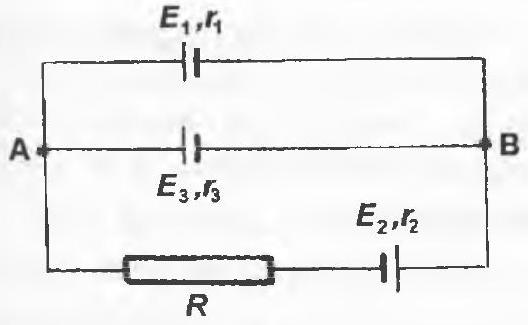
\includegraphics[max width=\textwidth, center]{2025_07_01_5b3ff9fa0d508c8e9f17g-147(1)} Fig. 3.2\\

3.19. Pe soclul unui bec este scris: $U=120 \mathrm{~V}, P=60 \mathrm{~W}$. Pentru a-l putea alimenta la tensiunea $U_{1}=220 \mathrm{~V}$ trebuie introdusă în circuit o rezistență adițională egală cu :\\ A) $100 \Omega$; B) $150 \Omega$; C) $200 \Omega$; D) $250 \Omega$; E) $300 \Omega$; F) $500 \Omega$.\\ (Gabriela Cone)\\

3.20. Tensiunea electrică de la bornele rezistorului $R$ din circuitul din Fig. 3.3 are valoarea ( $E_{1}=12 \mathrm{~V} ; E_{2}=6 \mathrm{~V} ; r_{1}=0,5 \Omega ; r_{2}=2 / 3 \Omega ; R=1 \Omega$ ):\\ A) $5,0 \mathrm{~V}$; B) $6,28 \mathrm{~V}$; C) $7,33 \mathrm{~V}$; D) $9,16 \mathrm{~V}$; E) $12 \mathrm{~V}$; F) $6,33 \mathrm{~V}$.\\ (Gabriela Cone)\\ 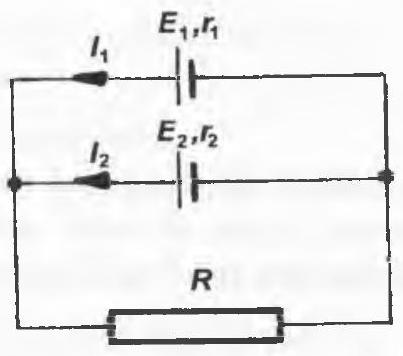
\includegraphics[max width=\textwidth, center]{2025_07_01_5b3ff9fa0d508c8e9f17g-147} Fig. 3.3\\

3.21. Puterea electrică $P=100 \mathrm{~kW}$ trebuie transmisă la distanța $d=100 \mathrm{~km}$ prin conductoare de cupru cu diametrul $D=2 \mathrm{~mm}$ astfel ca pierderile de putere să fie cel mult $2 \%\left(\rho_{\mathrm{Cu}}=1,75 \cdot 10^{-8} \Omega \mathrm{~m}\right)$. Tensiunea electrică sub care trebuie transmisă această putere este egală cu :\\ A) $75,4 \mathrm{kV}$; B) $65,2 \mathrm{kV}$; C) $100 \mathrm{~kV}$; D) $32 \mathrm{~kV}$; E) $87 \mathrm{~kV}$; F) $125 \mathrm{~V}$.\\ (Gabriela Cone)\\

3.22. Un conductor omogen, de forma unui cerc, are rezistența electrică $R=8 \Omega$. Punctele A şi B împart conductorul în două arce $\mathrm{AC}_{1} \mathrm{~B}$ şi $\mathrm{AC}_{2} \mathrm{~B}$, ale căror lungimi se află în raportul $1 / 3$. Un curent $I=4 \mathrm{~A}$ intră prin A şi iese prin B. Diferența de potențial dintre punctele $A$ şi $B$ este egală cu :\\ A) $6 \mathrm{~V}$; B) $7,5 \mathrm{~V}$; C) $10 \mathrm{~V}$; D) $12 \mathrm{~V}$; E) $13 \mathrm{~V}$; F) $21 \mathrm{~V}$.\\ (Gabriela Cone)\\

3.23. Un aparat de măsură cu rezistența $r_{0}=9,8 \Omega$ permite trecerea unui curent electric de intensitate $i_{0}=0,1 \mathrm{~A}$. Valoarea rezistenței adiționale $r_{a}$, care trebuie legată în serie cu aparatul pentru ca acesta să poată fi folosit ca voltmetru, care să măsoare tensiuni până la $30 \mathrm{~V}$, are valoarea :\\ A) $4 \Omega$; B) $100 \Omega$; C) $128,5 \Omega$; D) $290,2 \Omega$; E) $732,8 \Omega$; F) $210 \Omega$.\\ (Gabriela Cone)\\

3.24. Puterea maximă debitată în exterior de o baterie cu un număr $n=5$ de elemente legate în serie, având fiecare tensiunea electromotoare $E=1,4 \mathrm{~V}$ şi rezitența internă $r=0,3 \Omega$, pe o rezistentă $R$, are valoarea :\\ A) $5 \mathrm{~W}$; B) $2,15 \mathrm{~W}$; C) $8,16 \mathrm{~W}$; D) $7 \mathrm{~W}$; E) $6,72 \mathrm{~W}$; F) $3,53 \mathrm{~W}$.\\ (Gabriela Cone)\\

3.25. Două rezistoare având caracteristicile $R_{1}=40 \mathrm{k} \Omega, P_{1}=4 \mathrm{~W}$, respectiv $R_{2}=10 \mathrm{k} \Omega$ şi $P_{2}=4 \mathrm{~W}$ sunt legate în serie. Tensiunea electrică maximă care poate fi aplicată ansamblului celor două rezistoare are valoarea:\\ A) $220 \mathrm{~V}$; B) $440 \mathrm{~V}$; C) $500 \mathrm{~V}$; D) $550 \mathrm{~V}$; E) $700 \mathrm{~V}$; F) $900 \mathrm{~V}$.\\ (Gabriela Cone)\\

3.26. O sursă electrică, cu tensiunea electromotoare de $24 \mathrm{~V}$, este formată din $n$ elemente electrice înseriate, având fiecare rezistență electrică de $0,4 \Omega$. La bornele sale se conectează un rezistor $R$ prin care trece un curent de intensitate $I_{1}=2 \mathrm{~A}$. Dacă se scurtcircuitează jumătate din numărul de elemente ale sursei intensitatea curentului scade la valoarea $I_{2}=1,5 \mathrm{~A}$. Numărul de elemente $n$ al sursei este egal cu:\\ A) 5; B) 10; C) 15; D) 20; E) 30; F) 25.\\ (Gabriela Cone)\\

3.27. O baterie formată din elemente galvanice, având fiecare o tensiune electromotoare $E=1,9 \mathrm{~V}$ şi o rezistență interioară $r=0,1 \Omega$, trebuie să alimenteze două circuite electrice independente cu rezistențele $R_{1}=3 \Omega$ şi $R_{2}=10 \Omega$. Pentru ca prin cele două circuite să treacă acelaşi curent electric $I=2 \mathrm{~A}$, acestea trebuie legate la sursă:\\ A) în serie; B) în paralel; C) în circuite separate; D) una în serie şi cealaltă în paralel; E) o parte din $R_{2}$ în paralel cu $R_{1}$ şi restul în serie; F) nu este posibilă realizarea condiției din enunţ.\\ (Gabriela Cone)\\

3.28. În paralel cu un bec cu puterea $P_{1}=100 \mathrm{~W}$ este legat un reşou cu puterea $P_{2}=400 \mathrm{~W}$. Tensiunea electrică de la rețea este $U=220 \mathrm{~V}$, iar firele de legătură au rezistența $R=21 \Omega$. Prin legarea reşoului în circuit, tensiunea electrică la bornele becului:\\ A) creşte; B) rămâne constantă; C) scade; D) se anulează; E) tinde la infinit; F) îşi schimbǎ polaritatea.\\ (Gabriela Cone)\\

3.29. Rezistența electrică echivalentă a circuitului din Fig. 3.4 între punctele A şi B are valoarea:\\ A) $2 R$; B) $R$; C) $5 R$; D) $3 R$; E) $4 R$; F) $R / 2$.\\ (Gabriela Cone)\\ 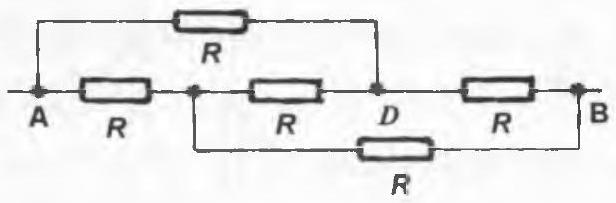
\includegraphics[max width=\textwidth, center]{2025_07_01_5b3ff9fa0d508c8e9f17g-149} Fig. 3.4\\

3.30. Două surse $E_{1}$ şi $E_{2}=125 \mathrm{~V}$, cu rezistența internă $r_{2}=0,2 \Omega$, sunt legate în paralel cu rezistența $R=2 \Omega$. Pentru ca intensitatea curentului $I_{1}$ prin sursa 1 să fie nulă tensiunea electromotoare $E_{1}$ trebuie să aibă valoarea:\\ A) $110 \mathrm{~V}$; B) $113,6 \mathrm{~V}$; C) $127,2 \mathrm{~V}$; D) $130 \mathrm{~V}$; E) $139 \mathrm{~V}$; F) $220 \mathrm{~V}$.\\ (Gabriela Cone)\\

3.31. Fie un generator cu tensiunea electromotoare $E$ şi rezistența internă $r$ şi două voltmetre identice de rezistență interioară $r_{V}$. Când un voltmetru este montat la bornele generatorului el indică $V_{1}$; când se adaugă al doilea voltmetru în paralel indicația lor comună este $V_{2}$. Expresia tensiunii electromotoare $E$ în funcție de $V_{1}$ şi $V_{2}$ este:\\ A) $\frac{V_{1} V_{2}}{2 V_{1}-V_{2}}$; B) $\frac{V_{1} V_{2}}{2 V_{2}-V_{1}}$; C) $\frac{V_{1} V_{2}}{V_{2}-V_{1}}$; D) $\frac{V_{1} V_{2}}{V_{1}-V_{2}}$; E) $\frac{V_{1} V_{2}}{2 V_{2}+V_{1}}$; F) $\frac{V_{1} V_{2}}{2 V_{1}+V_{2}}$.\\ (Daniela Buzatu)\\

3.32. Un circuit electric cuprinde un generator de tensiune electromotoare $E=4 \mathrm{~V}$ cu rezistența internă neglijabilă, un ampermetru cu rezistența internă neglijabilă şi două rezistoare $R_{1}=2 \Omega$ şi $R_{2}=4 \Omega$ legate în paralel. Intensitatea curentului indicată de ampermetru, precum şi intensitățile $I_{1}$ şi $I_{2}$ prin rezistențele $R_{1}$ şi respective $R_{2}$ sunt:\\ A) $4 \mathrm{~A} , 2 \mathrm{~A} , 2 \mathrm{~A}$; B) $5 \mathrm{~A} , 3 \mathrm{~A} , 2 \mathrm{~A}$; C) $3 \mathrm{~A} , 2 \mathrm{~A} , 1 \mathrm{~A}$; D) $6 \mathrm{~A} , 4 \mathrm{~A} , 2 \mathrm{~A}$; E) $6 \mathrm{~A} , 5 \mathrm{~A} , 1 \mathrm{~A}$; F) $2 \mathrm{~A} , 3 \mathrm{~A} , 1 \mathrm{~A}$.\\ (Daniela Buzatu)\\

3.33. De la o rețea de alimentare cu tensiunea la borne $U=20 \mathrm{kV}$ trebuie să se transmită la distanța $l=250 \mathrm{~km}$ puterea $P=500 \mathrm{~kW}$, cu o pierdere de tensiune $U^{\prime}$ pe linia bifilară de transport a energiei egală cu $12,5 \%$ din tensiunea $U$. Diametrul $\operatorname{minim} D$ al sârmei de cupru $\left(\rho=1,75 \cdot 10^{-8} \Omega \cdot \mathrm{~m}\right)$ pentru realizarea liniei de transport este:\\ A) $0,04 / \sqrt{\pi} \mathrm{m}$; B) $12,5 / \sqrt{\pi} \mathrm{m}$; C) $1,75 / \sqrt{\pi} \mathrm{m}$; D) $0,02 / \sqrt{\pi} \mathrm{m}$; E) $5 / \sqrt{\pi} \mathrm{m}$; F) $2,5 / \sqrt{\pi} \mathrm{m}$.\\ (Daniela Buzatu)\\

3.34. În circuitul electric din Fig. 3.5, se cunosc $R_{1}=4 \Omega ; R_{2}=6 \Omega$, $R_{3}=0,8 \Omega, R_{4}=0,6 \Omega, r=0,2 \Omega \quad E=24 \mathrm{~V}$. Curenții $I_{1}$ și $I_{2}$ prin rezistoarele $R_{1}$ şi $R_{2}$ au valorile:\\ A) $I_{1}=2,4 \mathrm{~A} , I_{2}=3,6 \mathrm{~A}$; B) $I_{1}=3,6 \mathrm{~A} , I_{2}=2,4 \mathrm{~A}$; C) $I_{1}=1,2 \mathrm{~A} , I_{2}=4,8 \mathrm{~A}$; D) $I_{1}=I_{2}=3 \mathrm{~A}$; E) $I_{1}=5 \mathrm{~A} , I_{2}=1 \mathrm{~A}$; F) $I_{1}=1 \mathrm{~A} , I_{2}=5 \mathrm{~A}$.\\ (Ilie Ivanov)\\ 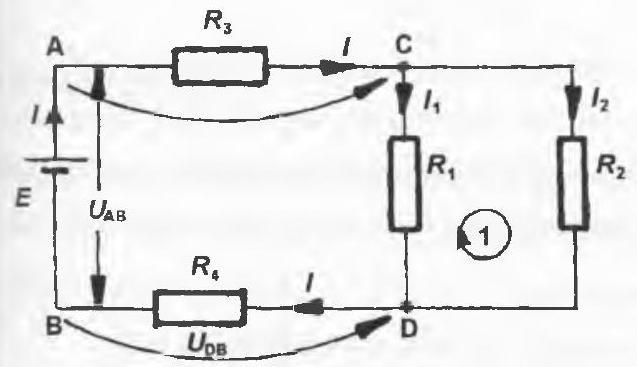
\includegraphics[max width=\textwidth, center]{2025_07_01_5b3ff9fa0d508c8e9f17g-151(3)} Fig. 3.5\\

3.35. În montajul din Fig. 3.6, $E=18 \mathrm{~V}, r=0, R=4 \Omega, R_{1}=6 \Omega, R_{2}=3 \Omega$. Curenții prin rezistențele $R_{1}$ şi $R_{2}$ au valorile:\\ A) $I_{1}=I_{2}=1,5 \mathrm{~A}$; B) $I_{1}=1,4 \mathrm{~A} , I_{2}=0,1 \mathrm{~A}$; C) $I_{1}=0,1 \mathrm{~A} , I_{2}=1,4 \mathrm{~A}$; D) $I_{1}=2 \mathrm{~A} , I_{2}=1 \mathrm{~A}$; E) $I_{1}=2,5 \mathrm{~A} , I_{2}=0,5 \mathrm{~A}$; F) $I_{1}=1 \mathrm{~A} , I_{2}=2 \mathrm{~A}$.\\ (Ilie Ivanov)\\ 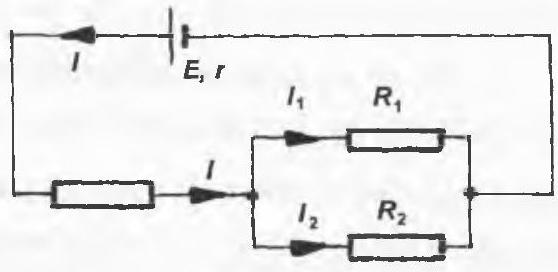
\includegraphics[max width=\textwidth, center]{2025_07_01_5b3ff9fa0d508c8e9f17g-151} Fig. 3.6\\

3.36. Rezistența echivalentă a montajului din Fig. 3.7 este:\\ A) $R / 2$; B) $2 R$; C) $7 R$; D) $3 R$; E) $R$; F) $R / 7$.\\ (Ilie Ivanov)\\ 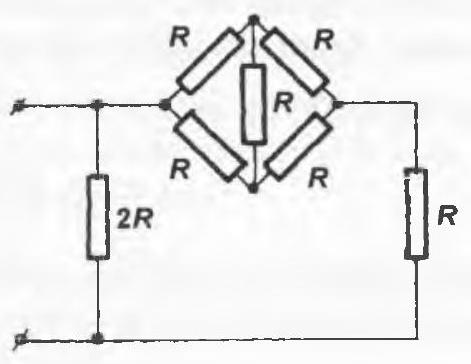
\includegraphics[max width=\textwidth, center]{2025_07_01_5b3ff9fa0d508c8e9f17g-151(2)} Fig. 3.7\\

3.37. O baterie electrică debitează pe o rezistență variabilă o putere ce reprezintă o fracțiune $f=46 \%$ din puterea maximă pe care ar putea să o debiteze. Se constată că există două valori ale tensiunii de la bornele bateriei pentru care se realizează acest lucru. Raportul celor două tensiuni este:\\ A) 2; B) $\sqrt{3}$; C) $\sqrt{2}$; D) 3; E) 6,54; F) 9.\\ (Mihai Cristea)\\

3.38. Un număr $n$ de pile electrice identice, de tensiune electromotoare $E$ şi rezistență internă $r$, sunt conectate ca în Fig. 3.8, ultima pilă fiind legată în opoziție față de celelalte. Curentul electric $I$ ce trece prin această pilă este:\\ A) $\frac{n+1}{n} \cdot \frac{2 E}{r}$; B) $\frac{n+1}{2 n} \cdot \frac{E}{r}$; C) $\frac{n-1}{2 n} \cdot \frac{E}{r}$; D) $\frac{n-1}{n} \cdot \frac{2 E}{r}$; E) $\frac{n^{2}-1}{n} \cdot \frac{E}{r}$; F) $\frac{n^{2}+1}{n} \cdot \frac{E}{r}$.\\ (Mihai Cristea)\\ 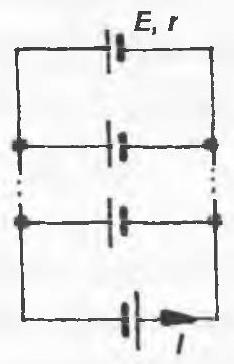
\includegraphics[max width=\textwidth, center]{2025_07_01_5b3ff9fa0d508c8e9f17g-151(1)} Fig. 3.8\\

3.39. Se conectează un rezistor la bornele unui generator de tensiune constantă și se găseşte un curent $I_{0}=35 \mathrm{~mA}$ când temperatura la care se află rezistorul este $t_{0}=0^{\circ} \mathrm{C}$. Dacă sistemul este adus la temperatura $t=100^{\circ} \mathrm{C}$, atunci curentul prin rezistor este $I=25 \mathrm{~mA}$. Coeficientul de variație termică a rezistivității este:\\ A) $5 \cdot 10^{-2} \mathrm{grad}^{-1}$; B) $4 \cdot 10^{-3} \mathrm{grad}^{-1}$; C) $6 \cdot 10^{-3} \mathrm{grad}^{-1}$; D) $3 \cdot 10^{-1}$ grad $^{-1}$; E) $5 \cdot 10^{-4} \mathrm{grad}^{-1}$; F) $1 \cdot 10^{-5} \mathrm{grad}^{-1}$.\\ (Mihai Cristea)\\

3.40. Două rezistoare de rezistențe $R_{1}=4 \Omega$ şi $R_{2}=6 \Omega$ se leagă în serie la o sursă de curent continuu. La legarea în paralel a rezistoarelor la aceeaşi sursă, curentul din circuitul principal creşte de trei ori. Rezistența internă a sursei este:\\ A) $2,8 \Omega$; B) $2,4 \Omega$; C) $1,8 \Omega$; D) $1,6 \Omega$; E) $1,4 \Omega$; F) $1,2 \Omega$.\\ (Mircea Stan)\\

3.41. Fie două baterii identice. Când se leagă în paralel cele două baterii la bornele unui rezistor având $R=16 \Omega$, intensitatea curentului în curentul principal este $I_{1}$. Dacă bateriile se leagă în serie la bornele aceluiași rezistor, intensitatea curentului din circuit devine $I_{2}=1,7 I_{1}$. Rezistenţa internă a unei baterii este:\\ A) $1 \Omega$; B) $2 \Omega$; C) $2,5 \Omega$; D) $3 \Omega$; E) $4,5 \Omega$; F) $5,2 \Omega$.\\ (Mircea Stan)\\

3.42. Un elev învață timp de 3 ore la lumina unui bec de $60 \mathrm{~W}$. Care este prețul energiei electrice consumate, dacă $1 \mathrm{~kWh}$ costă $1300 \mathrm{~lei}$ ?\\ A) $3900 \mathrm{~lei}$; B) $2400 \mathrm{~lei}$; C) $1800 \mathrm{~lei}$; D) $360 \mathrm{~lei}$; E) $234 \mathrm{~lei}$; F) $184 \mathrm{~lei}$.\\ (Mircea Stan)\\

3.43. Câți electroni trec intr-un minut printr-un conductor străbătut de un curent $I=0,64 \mathrm{~A}$ ? Sarcina electronului este $e=1,6 \cdot 10^{-19} \mathrm{C}$.\\ A) $9,6 \cdot 10^{19}$; B) $8,3 \cdot 10^{21}$; C) $24 \cdot 10^{19}$; D) $4,8 \cdot 10^{22}$; E) $6,2 \cdot 10^{21}$; F) $8,6 \cdot 10^{38}$.\\ (Mircea Stan)\\

3.44. Prin conectarea unui rezistor având $R=1400 \Omega$ la o sursă de curent continuu intensitatea curentului devine de 29 de ori mai mică decât intensitatea curentului de scurtcircuit. Rezistența internă a sursei este:\\ A) $15 \Omega$; B) $20 \Omega$; C) $25 \Omega$; D) $35 \Omega$; E) $50 \Omega$; F) $140 \Omega$.\\ (Mircea Stan)\\

3.45. O ghirlandă alcătuită din 50 de beculețe are puterea de $60 \mathrm{~W}$ şi este alimentată la $90 \mathrm{~V}$. Rezistența unui singur beculeț este:\\ A) $2,7 \Omega$; B) $3,8 \Omega$; C) $4,2 \Omega$; D) $6,3 \Omega$; E) $12,3 \Omega$; F) $30 \Omega$.\\ (Mircea Stan)\\

3.46. Când intrerupătorul K este deschis, rezistența echivalentă între punctele A şi B este $R$ (Fig. 3.9). Când întreupătorul K este închis, rezistența echivalentă între A şi B este $R^{\prime}$. Raportul $R / R^{\prime}$ este:\\ A) $\frac{128}{143}$; B) $\frac{236}{245}$; C) $\frac{123}{213}$; D) $\frac{215}{116}$; E) $\frac{246}{213}$; F) $\frac{126}{125}$.\\ (Mircea Stan)\\ 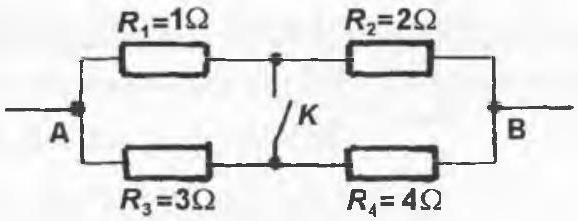
\includegraphics[max width=\textwidth, center]{2025_07_01_5b3ff9fa0d508c8e9f17g-153} Fig. 3.9\\

3.47. Printr-o sursă de tensiune electromotoare $E=24 \mathrm{~V}$ curentul de scurtcircuit are valoarea $I_{\mathrm{sc}}=60 \mathrm{~A}$. Rezistența ce trebuie conectată la bornele acesteia ca tensiunea la borne să fie $U=22 \mathrm{~V}$ are valoarea:\\ A) $5,4 \Omega$; B) $3,9 \Omega$; C) $5 \Omega$; D) $2,5 \Omega$; E) $4,4 \Omega$; F) $10 \Omega$.\\ (Constantin Neguțu)\\

3.48. Un element galvanic (sursă de tensiune electrică) cu rezistența internă de $0,2 \Omega$ are rezistența exterioară confecționată dintr-un fir de nichelină ( $\rho=4 \cdot 10^{-7} \Omega \mathrm{~m}$ ) lung de $6 \mathrm{~m}$ şi cu secțiunea de $1 \mathrm{~mm}^{2}$. La capetele firului se aplică o tensiune de $1,8 \mathrm{~V}$. Randamentul acestui circuit este:\\ A) 0,92; B) $0,92 \%$; C) $66 \%$; D) 0,67; E) $50 \%$; F) 1.\\ (Constantin Neguțu)\\

3.49. Se consideră un circuit electric simplu, format dintr-o sursă cu tensiunea electromotoare $E$ şi rezistența internă $r$, care alimentează un rezistor exterior cu rezistența $R$. Care din afirmațiile de mai jos este adevărată?\\ A) Intensitatea curentului prin circuit este $I=E(R+r)$; B) Căderea de tensiune pe rezistența internă a sursei este $u=\frac{r E}{R+r}$; C) Tensiunea la bornele sursei se poate scrie $U=\frac{E^{2}}{R+r}$; D) Intensitatea curentului la scurtcircuit este $I_{\mathrm{sc}}=\frac{E}{R}$; E) Puterea maximă debitată de sursă pe rezistența externă corespunde la $R=2 r$; F) Expresia puterii maxime debitate de sursă pe rezistenta exterioară este $P_{\max }=\frac{E^{2}}{8 r}$.\\ (Constantin Neguțu)\\

3.50. Se dă circuitul din Fig. 3.10. Condiția ca prin rezistorul $R$ să nu circule curent electric, oricare ar fi valoarea rezistenței sale, este:\\ A) $E_{1} r_{1}=E_{2} r_{2}$; B) $E_{1}=E_{2}$; C) $E_{1}>E_{2}$; D) $E_{1}<E_{2}$; E) $\frac{E_{1}}{r_{1}}>\frac{E_{2}}{r_{2}}$; F) $\frac{E_{1}}{r_{1}}=\frac{E_{2}}{r_{2}}$.\\ (Constantin Neguțu)\\ 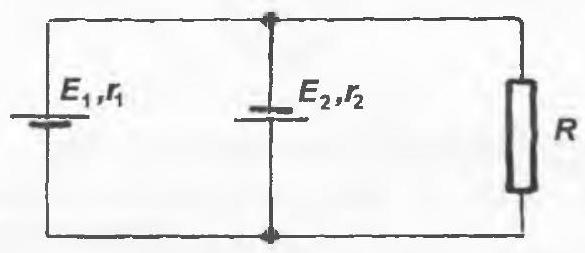
\includegraphics[max width=\textwidth, center]{2025_07_01_5b3ff9fa0d508c8e9f17g-154} Fig. 3.10\\

3.51. Intensitatea curentului electric ce trece printr-un conductor de cupru $\left(\rho_{\mathrm{Cu}}=1,7 \cdot 10^{-8} \Omega \mathrm{~m}\right)$ lung de $120 \mathrm{~m}$ şi cu secțiunea $6 \mathrm{~mm}^{2}$, dacă de-a lungul conductorului se produce o cădere de tensiune de $17 \mathrm{~V}$, are valoarea:\\ A) $17 \mathrm{~mA}$; B) $12 \mathrm{~A}$; C) $50 \mathrm{~A}$; D) $70 \mathrm{~mA}$; E) $3 \mathrm{~A}$; F) $0,1 \mathrm{~A}$.\\ (Gabriela Tiriba)\\

3.52. Un generator electric produce printr-o rezistență de $7 \Omega$ o putere electrică. Rezistența interioară a generatorului dacă acesta produce aceeaşi putere printr-o rezistență de $28 \Omega$ are valoarea:\\ A) $20 \Omega$; B) $14 \Omega$; C) $21 \mathrm{k} \Omega$; D) $7 \mathrm{k} \Omega$; E) $35 \mathrm{k} \Omega$; F) $40 \Omega$.\\ (Gabriela Tiriba)\\

3.53. Două surse cu tensiunea electromotoare de $12 \mathrm{~V}$ fiecare, cu rezistențele interioare de $1 \Omega$ şi respectiv de $1,5 \Omega$ sunt montate în paralel, prin prima sursă trecând un curent de $1,5 \mathrm{~A}$. Rezistența are circuitului exterior este?\\ A) $7 \Omega$; B) $4,2 \Omega$; C) $10,5 \Omega$; D) $8 \Omega$; E) $2,4 \Omega$; F) $7,5 \Omega$.\\ (Radu Chişleag)\\

3.54. La ce temperatură funcționează filamentul unui bec electric, dacă tensiunea de alimentare este de $120 \mathrm{~V}$, iar intensitatea este de $1 \mathrm{~A}$. La temperatura de $50^{\circ} \mathrm{C}$ rezistența filamentului becului este de $10 \Omega\left(\alpha=0,005 \mathrm{~K}^{-1}\right)$.\\ A) $3073 \mathrm{~K}$; B) $1937 \mathrm{~K}$; C) $2000^{\circ} \mathrm{C}$; D) $2500^{\circ} \mathrm{C}$; E) $3003 \mathrm{~K}$; F) $2457 \mathrm{~K}$.\\ (Radu Chişleag)\\

3.55. Un set de surse, identice având tensiunea electromotoare cunoscută şi rezistenta internă de $1 \Omega$, sunt conectate la capetele unui rezistor de rezistență $1000 \mathrm{~m} \Omega$. Cum se modifică curentul care trece prin rezistor, când se trece de la montajul de alimentare cu sursele în serie la montajul cu sursele în paralel?\\ A) scade de 10 ori; B) creşte de 1,1 ori; C) creşte de 2 ori; D) este acelaşi; E) creşte de 10 ori; F) scade de 2 ori.\\ (Radu Chişleag)\\

3.56. O sursă, cu rezistența interioară de $0,5 \Omega$ alimentează optim un consumator cu puterea de $100 \mathrm{~W}$. Tensiunea electromotoare a sursei este:\\ A) $7,2 \mathrm{~V}$; B) $14,1 \mathrm{~V}$; C) $24 \mathrm{~V}$; D) $200 \mathrm{~V}$; E) $50 \mathrm{~V}$; F) $100 \mathrm{~V}$.\\ (Radu Chişleag)\\

3.57. Tensiunea aplicată la capetele unui conductor este de $0,18 \mathrm{kV}$. Conductorul este parcurs de o sarcină de $0,5 \mathrm{kC}$, într-un timp necunoscut. Ce cantitate de căldură se produce în conductor ?\\ A) $0,09 \mathrm{~M.u.S.I.}$; B) nu se poate determina; C) $0,090 \mathrm{~kW}$; D) $90 \mathrm{~kWh}$; E) $0,36 \mathrm{MJ}$; F) $2,7 \mathrm{~kJ}$.\\ (Radu Chişleag)\\

3.58. Ce reprezintă "amper" în fizică ?\\ A) unitatea de masă a intensității curentului electric în S.I.; B) curentul care trece prin două conductoare paralele aflate la distanța de $1 \mathrm{~m}$, în vid, între care se exercită o forță de interacțiune de $2 \cdot 10^{-7} \mathrm{~N} / \mathrm{m}$; C) numele unui fizician francez; D) codul de acces la toate programele de fizică pe calculator; E) mărimea cea mai importantă în definirea sarcinii electrice în S.I.; F) numele curenților electrici elementari din atomi.\\ (Radu Chişleag)\\

3.59. Două baterii identice, cu tensiunea electromotoare $E=10 \mathrm{~V}$ şi rezistența internă $r=2 \Omega$ sunt legate la un rezistor de rezistență $R=4 \Omega$. Intensitatea curentului prin rezistorul $R$ în cazul în care sursele sunt legate în serie, față de cazul în care acestea sunt legate în paralel este mai mare de un număr de ori egal cu:\\ A) 1,25; B) 2; C) 3; D) 0,5; E) 1; F) 0,33.\\ (Mădălina Puică)\\

3.60. Trei reşouri, de $100 \mathrm{~W}$ fiecare, sunt conectate la tensiunea de $100 \mathrm{~V}$ în toate combinațiile posibile: în serie, în paralel, sau două în paralel cu al treilea în serie. Raportul între puterea totală maximă şi puterea totală minimă care poate fi obținută este:\\ A) 3; B) 2,5; C) 9; D) 2; E) 4; F) 10.\\ (Mădălina Puică)\\

3.61. O baterie de acumulatoare de $100 \mathrm{~V}$ are o rezistență internă de $5 \Omega$. Voltmetrul, având o rezistență de $500 \Omega$, indică când este legat la bornele bateriei o tensiune:\\ A) $99 \mathrm{~V}$; B) $0,9 \mathrm{kV}$; C) $0,66 \mathrm{kV}$; D) $95 \mathrm{~V}$; E) $100 \mathrm{~V}$; F) $90 \mathrm{~V}$.\\ (Ionuț Puică)\\

3.62. Un element galvanic cu rezistența internă $r$ debitează curent pe o rezistență de sarcină de valoare $R$. Puterea înregistrată pe rezistența $R$ este maximă dacă:\\ A) $R=3 r$; B) $R=1 \Omega$; C) $R=\max$; D) $R=r$; E) $R=0$; F) $R=2 / 3 r$.\\ (Marin Cilea)\\

3.63. Două elemente galvanice, identice, cu tensiunea electromotoare $E=2 \mathrm{~V}$ și rezistența internă $r$ se leagă în serie printr-un rezistor de rezistență $R=1 \Omega$. Intensitatea curentului ce străbate acest circuit, ştiind că o singură sursă ar debita prin rezistor un curent $I_{0}=2 \mathrm{~A}$, este:\\ A) $2 \mathrm{~A}$; B) $4 \mathrm{~A}$; C) $6 \mathrm{~A}$; D) $3,2 \mathrm{~A}$; E) $1,5 \mathrm{~A}$; F) $5 \mathrm{~A}$.\\ (Marin Cilea)\\

3.64. Intensitatea curentului electric care trece printr-un conductor de cupru lung de $440 \mathrm{~m}$ şi cu secțiunea de $1,7 \mathrm{~mm}^{2}$, conectat la tensiunea de $220 \mathrm{~V}$, ştiind că de-a lungul conductorului se produce o cădere de tensiune de $5 \%$ ? $\left(\rho_{\mathrm{Cu}}=1,7 \cdot 10^{-8} \Omega \mathrm{~m}\right)$ este:\\ A) $2,5 \mathrm{~A}$; B) $1 \mathrm{~A}$; C) $2 \mathrm{~A}$; D) $5 \mathrm{~A}$; E) $7 \mathrm{~A}$; F) $3 \mathrm{~A}$.\\ (Marin Cilea)\\

3.65.* O depunere electrolitică de ioni monovalenți durează $t=48 \mathrm{~s}$. Dacă intensitatea curentului electric este constantă în acest timp, egală cu $0,4 \mathrm{~A}$, ştiind că sarcina elementară $e=1,6 \cdot 10^{-19} \mathrm{C}$, numărul de ioni care ajung la catod este:\\ A) $2,4 \cdot 10^{20}$; B) $0,4 \cdot 10^{20}$; C) $5,1 \cdot 10^{20}$; D) $0,82 \cdot 10^{20}$; E) $3,2 \cdot 10^{20}$; F) $1,2 \cdot 10^{20}$.\\ (Constantin P. Cristescu)\\

3.66.* Un cadru conductor de forma unui pătrat cu latura de $4 \mathrm{~cm}$, având o rezistență $R=2,8 \cdot 10^{-3} \Omega$, este situat în plan orizontal. Un câmp magnetic omogen de inducţie $0,7 \mathrm{~T}$ este orientat perpendicular pe planul cadrului. Câmpul se reduce la zero în mod uniform în timp de $0,8 \mathrm{~s}$. Energia disipată în cadru datorită tensiunii electromotoare induse este:\\ A) $250 \mu \mathrm{~J}$; B) $365 \mu \mathrm{~J}$; C) $840 \mu \mathrm{~J}$; D) $720 \mu \mathrm{~J}$; E) $180 \mu \mathrm{~J}$; F) $560 \mu \mathrm{~J}$.\\ (Constantin P. Cristescu)\\

3.67. În circuitul din Fig. 3.11. bateria are tensiunea electromotoare $E=12 \mathrm{~V}$ şi rezistență internă neglijabilă, iar $R_{1}=6000 \Omega$. Un voltmetru cu rezistență internă $R_{i}=6000 \Omega$ legat în paralel cu $R_{1}$ arată o tensiune de $9 \mathrm{~V}$. Rezistența $R_{2}$ este:\\ A) $500 \Omega$; B) $3500 \Omega$; C) $1000 \Omega$; D) $2500 \Omega$; E) $6000 \Omega$; F) $800 \Omega$.\\ (Constantin P. Cristescu)\\ 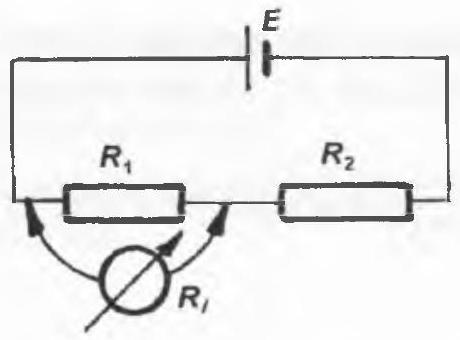
\includegraphics[max width=\textwidth, center]{2025_07_01_5b3ff9fa0d508c8e9f17g-158} Fig. 3.11\\

3.68. O sursă cu tensiunea electromotoare $E=2 \mathrm{~V}$ şi rezistența internă $r$ debitează pe o rezistență $R=3 \Omega$ un curent $I=0,5 \mathrm{~A}$. Raportul dintre curenții pe care o baterie de două asemenea surse legate în serie, respectiv în paralel, $I_{s} / I_{p}$, este:\\ A) $2 / 3$; B) $7 / 5$; C) $3 / 4$; D) $8 / 5$; E) $5 / 3$; F) $3 / 5$.\\ (Constantin P. Cristescu)\\

3.69. Dacă la bornele unei baterii se conectează un rezistor cu rezistența $R_{1}=1 \Omega$, intensitatea curentului în circuit este $I_{1}=1 \mathrm{~A}$. Dacă se conectează la borne un alt rezistor curezistența $R_{2}=3 \Omega$, intensitatea curentului este $I_{2}=0,5 \mathrm{~A}$. Puterea debitată de baterie în circuitul exterior când acesta este compus din cele două rezistoare legate în serie este:\\ A) $1,5 \mathrm{~W}$; B) $4 / 5 \mathrm{~W}$; C) $5 / 4 \mathrm{~W}$; D) $16 / 25 \mathrm{~W}$; E) $3 / 4 \mathrm{~W}$; F) $2,5 \mathrm{~W}$.\\ (Constantin P. Cristescu)\\

3.70. Un cablu telefonic subteran, format din două fire identice, are undeva un scurtcircuit. Cablul telefonic are $5 \mathrm{~km}$ lungime. Pentru a descoperi scurtcircuitul, un tehnician măsoară rezistența între terminalele A şi B şi obține $30 \Omega$ şi apoi între C şi D şi obține $70 \Omega$ (Fig. 3.12). Scurtcircuitul se află la distanța:\\ A) $1,5 \mathrm{~km}$ de A; B) $1,5 \mathrm{~km}$ de C; C) $3 \mathrm{~km}$ de B; D) $3 \mathrm{~km}$ de A; E) $3 \mathrm{~km}$ de C; F) $1,5 \mathrm{~km}$ de D.\\ (Alexandrina Nenciu)\\ 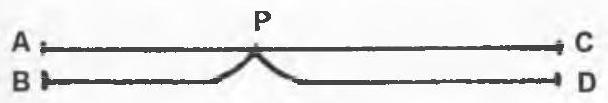
\includegraphics[max width=\textwidth, center]{2025_07_01_5b3ff9fa0d508c8e9f17g-159} Fig. 3.12\\

3.71. Două baterii cu tensiuni electromotoare $E_{1}=6 \mathrm{~V}$ şi $E_{2}=3 \mathrm{~V}$ sunt conectate la trei rezistențe cu valorile $R_{1}=6 \Omega, R_{2}=4 \Omega$ şi $R_{3}=2 \Omega$, ca în Fig. 3.13. Intensitatea curentului care trece prin fiecare baterie are valoarea:\\ A) $I_{3}=1 \mathrm{~A}, I_{4}=5,25 \mathrm{~A}$; B) $I_{3}=5,5 \mathrm{~A}, I_{4}=5,25 \mathrm{~A}$; C) $I_{3}=1 \mathrm{~A}, I_{4}=0,75 \mathrm{~A}$; D) $I_{3}=4,5 \mathrm{~A}, I_{4}=1 \mathrm{~A}$; E) $I_{3}=5,5 \mathrm{~A}, I_{4}=0,75 \mathrm{~A}$; F) $I_{3}=4,5 \mathrm{~A}, I_{4}=5,25 \mathrm{~A}$.\\ (Alexandrina Nenciu)\\ 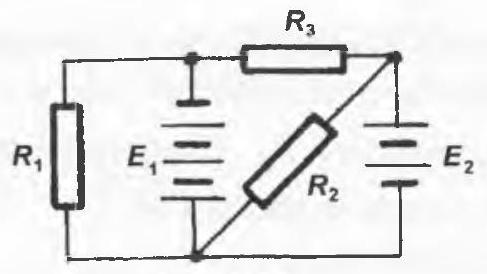
\includegraphics[max width=\textwidth, center]{2025_07_01_5b3ff9fa0d508c8e9f17g-159(2)} Fig. 3.13\\

3.72. O sursă cu tensiunea electromotoare $E$ şi rezistența $r$, dă unui rezistor conectat la bornele ei o putere $P$. Să se indice dacă acest lucru este posibil în cazul când:\\ A) valoarea rezistenței este unică; B) valoarea rezistenței este $R=r$; C) valoarea rezistenței este $R=\frac{r}{2}$; D) valoarea rezistenței poate fi oricare; E) există două valori ale rezistenței $R_{1}$ şi $R_{2}$ astfel încât $r=\sqrt{R_{1} R_{2}}$; F) există două valori ale rezistenței astfel încât $r=R_{1}+R_{2}$.\\ (Gheorghe Stanciu)\\

3.73. În circuitul din Fig. 3.14. voltmetrul indică tensiunea $U$, iar ampermetrul intensitatea $I$. Neglijând rezistența ampemetrului să se arate cǎ rezistența voltmetrului $R_{V}$ este (în voltmetru intensitatea curentului este neglijabilă):\\ A) $R_{V}=\frac{U}{I}$; B) $R_{V}=\frac{R U}{R I-U}$; C) $R_{V}=\frac{U+R I}{I}$; D) $R_{V}=\frac{R I-U}{I}$; E) $R_{V}=R$; F) $R_{V}=\frac{1}{2} \frac{U-R I}{I}$.\\ (Gheorghe Stanciu)\\ 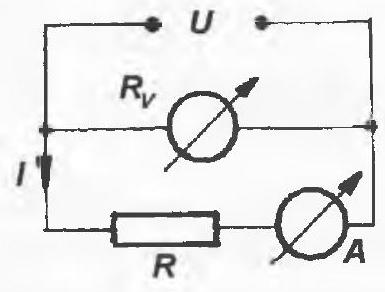
\includegraphics[max width=\textwidth, center]{2025_07_01_5b3ff9fa0d508c8e9f17g-159(1)} Fig. 3.14.\\

3.74. Două fire cu aceeaşi secțiune şi lungime, dar confecționate din materiale diferite, cu rezistivitățile $\rho_{01}$ şi $\rho_{02}$, au coeficienții de temperatură ai rezistivității $\alpha_{1}$ respectiv $\alpha_{2}$. Coeficientul de temperatură al sistemului obținut din cele două fire legate în paralel este:\\ A) $\alpha_{\text {paralel }}=\frac{\rho_{01} \alpha_{2}+\rho_{02} \alpha_{1}}{\rho_{01}+\rho_{02}}$; B) $\alpha_{\text {paralel }}=\frac{\rho_{01} \rho_{02}}{\rho_{01}+\rho_{02}}$; C) $\alpha_{\text {paralel }}=\frac{\alpha_{2} \alpha_{1}}{\alpha_{1}+\alpha_{2}}$; D) $\alpha_{\text {paralel }}=\frac{\rho_{02} \alpha_{2}+\rho_{01} \alpha_{1}}{\rho_{01}+\rho_{02}}$; E) $\alpha_{\text {paralel }}=\frac{\rho_{01} \alpha_{2}-\rho_{02} \alpha_{1}}{\rho_{01}+\rho_{02}}$; F) $\alpha_{\text {paralel }}=\frac{\rho_{01} \alpha_{2}-\rho_{02} \alpha_{1}}{\rho_{01}-\rho_{02}}$.\\ (Constantin Roşu)\\

3.75. Două baterii cu aceeaşi tensiune electromotoare au randamente $\eta_{1}$, respectiv $\eta_{2}$, pe aceeaşi rezistență exterioară. În cazul legării în paralel a bateriilor, randamentul lor total $\eta$ va fi:\\ A) $\eta>\eta_{1} , \eta>\eta_{2}$; B) $\eta=\eta_{1} , \eta>\eta_{2}$; C) $\eta<\eta_{1} , \eta<\eta_{2}$; D) $\eta=\eta_{1} , \eta>\eta_{2}$; E) nu se poate da un răspuns doarece nu este precizată rezistența de sarcină; F) $\eta+\eta_{1}>1 , \eta<\eta_{2}$.\\ (Constantin Roşu)\\

3.76. In circuitul din Fig. 3.15 se cunosc $R_{1}=100 \Omega, R_{2}=200 \Omega$, $R_{3}=400 \Omega, E_{1}=5 \mathrm{~V}, E_{2}=15 \mathrm{~V}$, iar sursele nu au rezistență internă. Tensiunea electrică dintre punctele A şi B va fi:\\ A) $U=6,43 \mathrm{~V}$; B) $U=-10 \mathrm{~V}$; C) $U=2,5 \mathrm{~V}$; D) $U=0 \mathrm{~V}$; E) $U=12 \mathrm{~V}$; F) $U=16 \mathrm{~V}$.\\ (Constantin Roşu)\\ 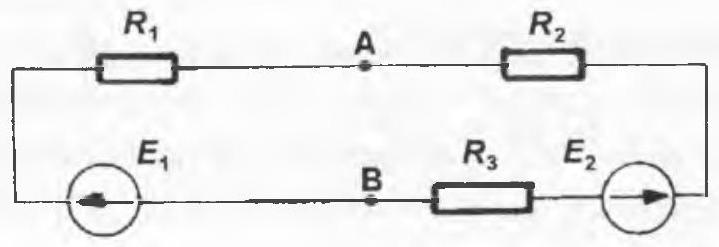
\includegraphics[max width=\textwidth, center]{2025_07_01_5b3ff9fa0d508c8e9f17g-160} Fig. 3.15.\\

3.77.* Sarcina electrică necesară pentru a depune $3 \mathrm{~moli}$ de produs biatomic prin electroliză este:\\ A) $\frac{21}{5} e N_{A}$; B) $\frac{3}{2} F$; C) $\frac{7}{5} N_{A}$; D) $3 e N_{A}$; E) $2 F$; F) $4 F$.\\ (Constantin Roşu)\\

3.78. Cantitatea $1 \mathrm{~CV}$ este echivalentă cu:\\ A) $1 \mathrm{~J}$; B) $1 \mathrm{~V} / \mathrm{m}$; C) $1 \mathrm{~N} / \mathrm{m}^{2}$; D) $1 \mathrm{C} / \mathrm{N}$; E) $1 F$; F) $1 W$.\\ (Alexandru Lupaşcu)\\

3.79. O sursă cu tensiunea electromotoare de  $12 \mathrm{~V}$ și rezistența internă de $0,2 \Omega$ debitează pe o rezistență variabilă. Rezistența este variată până când disipează o putere maximă. Intensitatea curentului care o străbate în acest caz este:\\ A)  $60 \mathrm{~A}$; B) $12 \mathrm{~A}$; C) $30 \mathrm{~A}$; D) $2,4 \mathrm{~A}$; E) $4,8 \mathrm{~A}$; F) $24 \mathrm{~A}$.\\ (Alexandru Lupaşcu)\\

3.80. La bornele unei surse se leagă în serie două voltmetre care indică tensiunile $U_{1}=8 \mathrm{~V}$ şi $U_{2}=6 \mathrm{~V}$. Dacă se leagă numai al doilea voltmetru, acesta indică tensiunea $U_{2}^{\prime}=10 \mathrm{~V}$. Tensiunea electromotoare a sursei este:\\ A) $20 \mathrm{~V}$; B)  $7 \mathrm{~V}$; C)  $17 \mathrm{~V}$; D)  $22 \mathrm{~V}$; E)  $18 \mathrm{~V}$; F) altă valoare.\\ (Alexandru Lupaşcu)\\

3.81. O sursă disipează în circuitul exterior aceeași putere $P=80 \mathrm{~W}$ când la borne este legat un rezistor cu rezistența $R_{1}=5 \Omega$ sau unul cu $R_{2}=20 \Omega$. Rezistența internă a sursei şi tensiunea electromotoare a ei au valorile :\\ A) $r=100 \Omega, E=94 \mathrm{~V}$; B) $r=10 \Omega, E=60 \mathrm{~V}$; C) $r=1 \Omega, E=53,66 \mathrm{~V}$; D) $r=10 \Omega, E=20 \mathrm{~V}$; E) $r=1 \Omega, E=20 \mathrm{~V}$; F) $r=1 \Omega, E=94 \mathrm{~V}$.\\ (Tatiana Pop)\\

3.82. Un ampermetru pentru măsurarea curenților foarte mici are rezistența de $150 \Omega$ şi poate măsura curenți până la $10 \mathrm{~mA}$. Pentru a putea folosi acest ampermetru la măsurarea curenților de $1 \mathrm{~A}$ trebuie introdusă în schema aparatului o rezistență egală cu:\\ A) $15,5 \Omega$; B) $150 \Omega$; C) $151,5 \Omega$; D) $1,515 \Omega$; E) $10 \Omega$; F) $1 \mathrm{M} \Omega$.\\ (Tatiana Pop)\\

3.83. Dacă se aplică o tensiune de $6 \mathrm{~V}$ între punctele diametral opuse ale unui inel conductor, puterea disipată este de $9,0 \mathrm{~W}$. Aplicând aceeaşi tensiune între două puncte A şi B ale inelului, puterea disipată devine $9,6 \mathrm{~W}$. Rezistențele electrice ale celor două arce de inel cuprinse între punctele A şi B sunt:\\ A) $9 \Omega , 7 \Omega$; B) $10 \Omega , 6 \Omega$; C) $11 \Omega , 5 \Omega$; D) $5 \Omega , 11 \Omega$; E) $7 \Omega , 9 \Omega$; F) $9 \Omega , 11 \Omega$.\\ (Tatiana Pop)\\

3.84. Două surse de tensiuni electromotoare $E_{1}$ şi respectiv $E_{2}=100 \mathrm{~V}$, au rezistențele interne $r_{1}=0 \Omega$ şi respectiv $r_{2}=0,2 \Omega$. Sursele sunt legate în paralel cu o rezistență $R=1,8 \Omega$. Pentru ca intensitatea curentului prin sursa de tensiune $E_{1}$ să fie nulă, tensiunea electromotoare a acestei surse trebuie să fie egală cu:\\ A) $110 \mathrm{~V}$; B) $114 \mathrm{~V}$; C) $90 \mathrm{~V}$; D) $139 \mathrm{~V}$; E) $45 \mathrm{~V}$; F) $120 \mathrm{~V}$.\\ (Elena Slavnicu)\\

3.85. Trei rezistențe de valori $R_{1}=1 \Omega, R_{2}=2 \Omega$ şi $R_{3}=3 \Omega$ sunt legate în toate modurile posibile. Produsul dintre valoarea minimă și valoarea maximă a rezistenței grupului este:\\ A) $\frac{8}{5} \Omega^{2}$; B) $4 \Omega^{2}$; C) $10 \Omega^{2}$; D) $\frac{36}{11} \Omega^{2}$; E) $\frac{23}{12} \Omega^{2}$; F) $6 \Omega^{2}$.\\ (Elena Slavnicu)\\

3.86. Într-un circuit cu rezistența $R$ o baterie are randamentul $\eta_{1}=0,3$. În același circuit, o altă baterie are randamentul $\eta_{2}=0,5$. Randamentul celor două baterii legate în serie, în circuitul cu rezistența $R$, va fi:\\ A) 0,2; B) 0,3; C) 0,4; D) 0,27; E) 0,23; F) 0,05.\\ (Maria Honciuc)\\

3.87. Intensitatea de scurtcurcuit a unui generator este $I_{0}=10 \mathrm{~A}$. Realizânduse un circuit electric cu acest generator, intensitatea curentului in circuit este $I=2 \mathrm{~A}$. Randamentul circuitului este:\\ A) 0,3; B) 0,65; C) 0,8; D) 0,7; E) 0,5; F) 0,25.\\ (Maria Honciuc)\\

3.88. Un circuit electric constă dintr-un ansamblu de trei rezistoare în serie, conectate la o baterie de $24 \mathrm{~V}$. Curentul prin circuit este de $0,032 \mathrm{~A}$. ştiind că $R_{1}=250 \Omega$ şi $R_{2}=150 \Omega$, căderile de tensiune pe fiecare rezistor sunt:\\ A) $U_{1}=4,8 \mathrm{~V} , U_{2}=8 \mathrm{~V} , U_{3}=11,2 \mathrm{~V}$; B) $U_{1}=8 \mathrm{~V} , U_{2}=4,2 \mathrm{~V} , U_{3}=11,8 \mathrm{~V}$; C) $U_{1}=4 \mathrm{~V} , U_{2}=8,8 \mathrm{~V} , U_{3}=11,2 \mathrm{~V}$; D) $U_{1}=10 \mathrm{~V} , U_{2}=4,8 \mathrm{~V} , U_{3}=11,2 \mathrm{~V}$; E) $U_{1}=8 \mathrm{~V} , U_{2}=4,8 \mathrm{~V} , U_{3}=11,2 \mathrm{~V}$; F) $U_{1}=4 \mathrm{~V} , U_{2}=4,2 \mathrm{~V} , U_{3}=4,8 \mathrm{~V}$.\\ (Cristina Stan)\\

3.89. Două becuri identice sunt conectate la aceeaşi baterie, prima dată în serie și apoi în paralel. Becurile grupate în serie vor disipa o putere ( $r=0$ ):\\ A) de 2 ori mai mare; B) de 2 mai mică; C) de 4 ori mai mică; D) egală; E) de 4 ori mai mare; F) de 3 ori mai mare decât cele grupate în paralel.\\ (Cristina Stan)\\

3.90. Circuitul electric din Fig. 3.16. constă într-un ansamblu de două rezistoare grupate in serie conectate la o baterie de $24 \mathrm{~V}$. Dacă curentul care circulă prin rezistorul de $6 \Omega$ are intensitatea de $1 \mathrm{~A}$, curentul care circulă prin rezistorul de $18 \Omega$ are intensitatea:\\ A) $3 \mathrm{~A}$; B) $0,3 \mathrm{~A}$; C) $1 \mathrm{~A}$; D) $5,33 \mathrm{~A}$; E) $1,3 \mathrm{~A}$; F) $2,1 \mathrm{~A}$.\\ (Cristina Stan)\\ 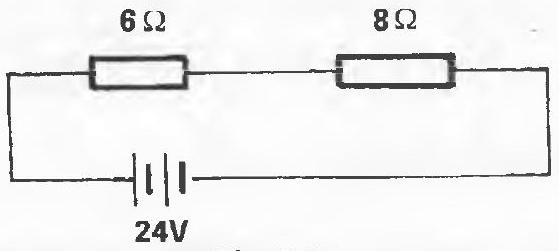
\includegraphics[max width=\textwidth, center]{2025_07_01_5b3ff9fa0d508c8e9f17g-163} Fig. 3.16\\

3.91. Două consumatoare care la tensiunea nominalǎ $U$ dezvoltă puterile $P_{1}=200 \mathrm{~W}$ şi $P_{2}=400 \mathrm{~W}$ sunt legate în paralel, apoi în serie. Raportul dintre căldurile degajate în timpul $\tau$ va fi:\\ A) $\frac{W_{p}}{W_{s}}=2$; B) $\frac{W_{p}}{W_{s}}=4$; C) $\frac{W_{p}}{W_{s}}=\frac{1}{2}$; D) nu se poate calcula pentru că nu se cunoaşte $U$; E) $\frac{W_{p}}{W_{s}}=4,5$; F) $\frac{W_{p}}{W_{s}}=\frac{1}{4,5}$.\\ (Rodica Bena)\\

3.92. Se leagă $n$ rezistoare diferite, o dată în serie, apoi în paralel. Raportul $\frac{R_{s}}{R_{p}}$ este:\\ A) $\frac{R_{s}}{R_{p}}=n^{2}$; B) $\frac{R_{s}}{R_{p}}<n^{2}$; C) $\frac{R_{s}}{R_{p}}>n^{2}$; D) $\frac{R_{s}}{R_{p}}=\frac{1}{n^{2}}$; E) $\frac{R_{s}}{R_{p}}>\frac{1}{n^{2}}$; F) $\frac{R_{S}}{R_{p}}=n(n+1)$.\\ (Rodica Bena)\\

3.93. Într-un circuit format dintr-o baterie şi un reostat curentul electric este $I$. Dacă se micşorează rezistența reostatului de $k$ ori, curentul creşte de $n$ ori. Intensitatea curentului de scurtcircuit este:\\ A) $I_{0}=I \frac{(k-1)}{n(k-n)}$; B) $I_{0}=I \frac{n(k-1)}{k-n}$; C) $I_{0}=I \frac{k}{n}$; D) $I_{0}=I \frac{n(k-n)}{k-1}$; E) $I_{0}=I \frac{k-n}{n(k-1)}$; F) $I_{0}=I \frac{k n-1}{k-n}$.\\ (Mona Mihăilescu)\\

3.94. Circuitul din Fig. 3.17 este alimentat la o baterie alcătuită din $n=10$ elemente galvanice legate în serie, având fiecare tensiunea electromotoare $e=2 \mathrm{~V}$ şi rezistența internă $r=0,1 \Omega$. Intensitatea $I$ a curentului principal este:\\ A) $I=0,4 \mathrm{~A}$; B) $I=4,8 \mathrm{~A}$; C) $I=2 \mathrm{~A}$; D) $I=1,58 \mathrm{~A}$; E) $I=4 \mathrm{~A}$; F) $I=10 \mathrm{~A}$.\\ (Mona Mihăilescu)\\ 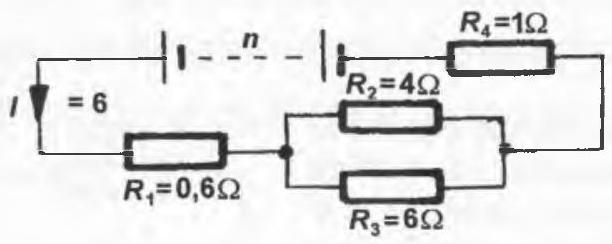
\includegraphics[max width=\textwidth, center]{2025_07_01_5b3ff9fa0d508c8e9f17g-164} Fig. 3.17\\

3.95. Un generator electric debitează pe rezistorul $R_{1}$ puterea $P_{1}$, iar pe rezistorul $R_{2}$ puterea $P_{2}=P_{1}$. Rezistența internă a generatorului în funcție de $R_{1}$ şi $R_{2}$ are expresia:\\ A) $\sqrt{R_{1}-R_{2}}$; B) $\sqrt{R_{1}+R_{2}}$; C) $\sqrt{R_{1} R_{2}}$; D) $\frac{R_{1}+R_{2}}{2}$; E) $\frac{R_{1}-R_{2}}{2}$; F) $\sqrt{\frac{R_{1}+R_{2}}{2}}$.\\ (Mona Mihăilescu)\\

3.96. O sursă cu tensiunea electromotoare $E$ şi rezistență interioară $r$ disipă în circuitul exterior aceeaşi putere $P=80 \mathrm{~W}$ când la borne este legat un rezistor cu rezistența $R_{1}=5 \Omega$ sau un rezistor cu rezistența $R_{2}=20 \Omega$. Tensiunea electromotoare a sursei este:\\ A) $25 \mathrm{~V}$; B) $30 \mathrm{~V}$; C) $80 \mathrm{~V}$; D) $16 \mathrm{~V}$; E) $60 \mathrm{~V}$; F) $75 \mathrm{~V}$.\\ (Ion Belciu)\\

3.97. Două voltmetre care pot măsura $150 \mathrm{~V}$, unul având rezistența de $15000 \Omega$ şi altul având rezistența de $150000 \Omega$ sunt conectate în serie la o rețea cu tensiunea $U=120 \mathrm{~V}$. Tensiunea indicată de fiecare voltmetru este:\\ A) $10,9 \mathrm{~V}$ şi $109,1 \mathrm{~V}$; B) $1 \mathrm{~V}$ şi $10 \mathrm{~V}$; C) $100 \mathrm{~V}$ şi $10 \mathrm{~V}$; D) $2 \mathrm{~V}$ şi $129,1 \mathrm{~V}$; E) $11,9 \mathrm{~V}$ şi $129,1 \mathrm{~V}$; F) $10 \mathrm{~V}$ şi $150 \mathrm{~V}$.\\ (Ileana Creangă)\\

3.98. Un rezistor cu rezistența de $60 \Omega$ şi altul cu rezistența de $90 \Omega$ sunt legate in paralel, iar montajul este conectat la o rețea cu tensiunea $U=120 \mathrm{~V}$. Intensitatea curentului total precum şi intensitatea curentului prin fiecare rezistor au valorile:\\ A) $I=3,33 \mathrm{~A} , I_{1}=2 \mathrm{~A} , I_{2}=1,33 \mathrm{~A}$; B) $I=33 \mathrm{~A} , I_{1}=1,2 \mathrm{~A} , I_{2}=3,3 \mathrm{~A}$; C) $I=3,33 \mathrm{~V} , I_{1}=2 \mathrm{~V} , I_{2}=1,33 \mathrm{~V}$; D) $I=3,33 \mathrm{~A} , I_{1}=12 \mathrm{~A} , I_{2}=13 \mathrm{~A}$; E) $I=33,3 \mathrm{~A} , I_{1}=12 \mathrm{~A} , I_{2}=33 \mathrm{~A}$; F) $I=3,03 \mathrm{~A} , I_{1}=1,2 \mathrm{~A} , I_{2}=1 \mathrm{~A}$.\\ (Ileana Creangă)\\

3.99.* Un voltametru cu azotat de argint şi electrozi de platină, având rezistența $R=1,9 \Omega$ și tensiunea contraelectromotoare de $1,2 \mathrm{~V}$, este alimentat de la un acumulator având tensiunea electromotoare de $2,2 \mathrm{~V}$ şi rezistența internă $r=0,1 \Omega$. Cantitatea de argint depusă în $30 \mathrm{~min}$ este (se dau pentru argint: masa atomică $A=107,8$ şi valența $n=1$ ):\\ A) $1 \mathrm{~kg}$; B) $0,5 \mathrm{~kg}$; C) $1 \mathrm{~g}$; D) $10 \mathrm{~g}$; E) $100 \mathrm{~g}$; F) $50 \mathrm{~g}$.\\ (Răzvan Mitroi)\\

3.100. Două rezistențe $R_{1}$ şi $R_{2}$ sunt montate în paralel şi alimentate de la o sursă cu $E=24 \mathrm{~V}$ şi rezistență interioară $r=1,2 \Omega$. Cunoscând rezistența $R_{1}=2 \Omega$, să se afle rezistența $R_{2}$ în cazul în care puterea absorbită în circuitul exterior este maximă.\\ A) $1,5 \Omega$; B) $3 \Omega$; C) $2 \Omega$; D) $5 \Omega$; E) 1,2; F) $3,2 \Omega$.\\ (Răzvan Mitroi)\\

3.101. Un încălzitor electric alimentat la o tensiune electrică de $220 \mathrm{~V}$ furnizează $4180 \mathrm{~kcal}$ pe oră. Valoarea rezistenței încălzitorului este ( $1 \mathrm{cal}=4,18 \mathrm{~J}$ ):\\ A) $10 \Omega$; B) $1 \Omega$; C) $20 \Omega$; D) $5 \Omega$; E) $2 \Omega$; F) $15 \Omega$.\\ (Vasile Popescu)\\

3.102. Pentru porțiunea de circuit din Fig. 3.18 se cunosc: $E_{1}=8 \mathrm{~V}$, $E_{2}=42 \mathrm{~V}, R_{1}=5 \Omega, R_{2}=8 \Omega, r_{1}=r_{2}=1 \Omega$ şi $I=3 \mathrm{~A}$. Diferenţa de potenţial $V_{\mathrm{A}}-V_{\mathrm{B}}$ este:\\ A) $80 \mathrm{~V}$; B) $-6,4 \mathrm{~V}$; C) $7 \mathrm{~V}$; D) $8,4 \mathrm{~V}$; E) $-11 \mathrm{~V}$; F) $-0,4 \mathrm{~V}$.\\ (Nicoleta Eşeanu)\\ 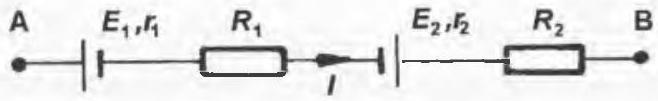
\includegraphics[max width=\textwidth, center]{2025_07_01_5b3ff9fa0d508c8e9f17g-166} Fig. 3.18\\

3.103. În circuitul din Fig. 3.19 se cunosc $E, R$ şi $r=9 R / 40$. Ampermetrul (ideal) indică:\\ A) $\frac{10 E}{21 R}$; B) $\frac{5 E}{12 R}$; C) $\frac{7 E}{2 R}$; D) $\frac{9 E}{13 R}$; E) $\frac{3 E}{17 R}$; F) nici o variantă nu este corectă.\\ (Nicoleta Eşeanu)\\ 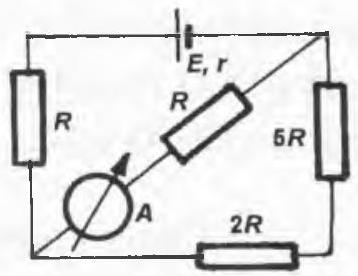
\includegraphics[max width=\textwidth, center]{2025_07_01_5b3ff9fa0d508c8e9f17g-166(1)} Fig. 3.19\\

3.104. Un ampermetru are rezistența internă $r=36 \Omega$ și scala de 150 diviziuni. La trecerea unui curent de $1 \mathrm{~A}$ acul ampermetrului deviază cu 50 diviziuni. Rezistența unui şunt legat în circuit astfel încât la trecerea unui curent de $5 \mathrm{~A}$ acul să devieze cu 10 diviziuni este:\\ A) $1,44 \Omega$; B) $1,5 \Omega$; C) $2,88 \Omega$; D) $3 \Omega$; E) $6 \Omega$; F) $6,8 \Omega$.\\ (Nicoleta Eşeanu)\\

3.105. Cursorul unui potentiometru de rezistentă $R=12 \mathrm{k} \Omega$ se află la o treime față de capătul notat A. Între cursor şi capătul A se leagă un voltmetru având rezistenta $R_{V}=16 \mathrm{k} \Omega$. Tensiunea de la bornele potențiometrului este $U=336 \mathrm{~V}$. Indicația voltmetrului este:\\ A) $96 \mathrm{~V}$; B) $72 \mathrm{~V}$; C) $162 \mathrm{~V}$; D) $124,5 \mathrm{~V}$; E) $31,8 \mathrm{~V}$; F) $63,6 \mathrm{~V}$.\\ (Nicoleta Eşeanu)\\

3.106. Un bec şi un reostat sunt legate în serie la o sursă de tensiune continuă astfel încât la bornele becului tensiunea este $60 \mathrm{~V}$. Rezistența reostatului este $60 \Omega$. Becul și reostatul consumă împreună $1200 \mathrm{~W}$. Intensitatea curentului în circuit este:\\ A) $5 \mathrm{~A}$; B) $2 \mathrm{~A}$; C) $2,8 \mathrm{~A}$; D) $8 \mathrm{~A}$; E) $4 \mathrm{~A}$; F) $8,6 \mathrm{~A}$.\\ (Nicoleta Eşeanu)\\

3.107. O sursă ideală având tensiunea electromotoare $E$ alimentează un circuit format din două rezistențe $R$ şi $5 R$ legate în paralel. Folosim aceeaşi sursă şi aceleaşi rezistoare, legate acum în serie. Raportul puterilor debitate de sursă în cele două cazuri este:\\ A) 1,2; B) $5 / 6$; C) 3,6; D) 7,2; E) 7; F) 4,2.\\ (Nicoleta Eşeanu)\\

3.108. Puterea dezvoltată în rezistența exterioară a unui circuit de curent continuu este $P=150 \mathrm{~W}$. Dacă mărim rezistența exterioară cu $80 \%$, puterea creşte cu $25 \%$. Valoare puterii dacă, în loc să mărim rezistența, o micşorăm cu $25 \%$ este:\\ A) $141 \mathrm{~W}$; B) $128 \mathrm{~W}$; C) $3,5 \mathrm{~kW}$; D) $85,5 \mathrm{~W}$; E) $103 \mathrm{~W}$; F) $206 \mathrm{~W}$.\\ (Nicoleta Eşeanu)\\

3.109. Un rezistor $R$ este alimentat, pe rând, la două surse de tensiune continuă. În primul caz randamentul de transmisie a puterii este $60 \%$, iar în al doilea caz este $40 \%$. Legăm cele două surse în serie la bornele aceluiaşi rezistor. Randamentul circuitului nou format este:\\ A) $49 \%$; B) $24 \%$; C) $46 \%$; D) $31,6 \%$; E) $54 \%$; F) $58,4 \%$.\\ (Nicoleta Eşeanu)\\

3.110. În circuitul din Fig. 3.20 rezistoarele sunt identice şi au valoarea $22 \Omega$, iar sursa are parametrii $E=150 \mathrm{~V}$ şi $r=1 \Omega$. Rezistența $R_{1}=4 \Omega$. Intensitatea curentului prin $R_{1}$ este :\\ A) $5 \mathrm{~A}$; B) $10 \mathrm{~A}$; C) $15 \mathrm{~A}$; D) $20 \mathrm{~A}$; E) $25 \mathrm{~A}$; F) nici o variantă nu este corectă.\\ (Nicoleta Eşeanu)\\ 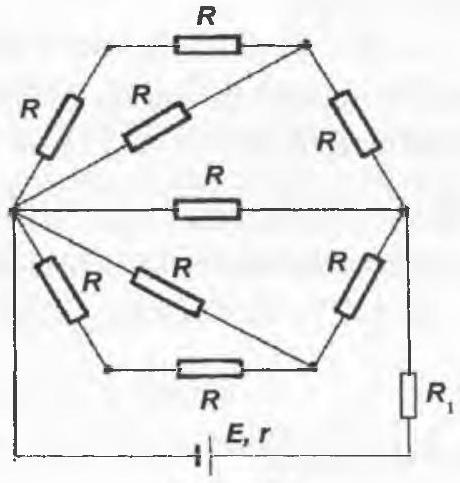
\includegraphics[max width=\textwidth, center]{2025_07_01_5b3ff9fa0d508c8e9f17g-167} Fig. 3.20\\

3.111. Două rezistoare au rezistențele $R$ și respectiv $4 R$ şi sunt alimentate la o sursă $(E, r)$ şi legate în paralel. Intensitatea curentului în sursă este egală cu?\\ A) $\frac{E}{R+r}$; B) $\frac{5 E}{4 R+5 r}$; C) $\frac{E}{5 R+r}$; D) 0; E) $\infty$; F) $\frac{4 E}{5 R+4 r}$.\\ (Nicoleta Eşeanu)\\

3.112. Un rezistor cu rezistența $R_{2}=10 \Omega$ este înseriat cu un rezistor $R_{1}=8 \Omega$ şi cu o sursă având $E=40 \mathrm{~V}$ şi $r=2 \Omega$. Intensitatea curentului în circuit este:\\ A) $2 \mathrm{~A}$; B) $1 \mathrm{~A}$; C) $0,5 \mathrm{~A}$; D) $0,25 \mathrm{~A}$; E) $3 \mathrm{~A}$; F) $10 \mathrm{~A}$.\\ (Nicoleta Eşeanu)\\

3.113. Un ampermetru cu rezistența $R_{\mathrm{A}}=1 \Omega$ este legat în paralel cu un conductor de cupru cu rezistivitatea $\rho=17 \cdot 10^{-9} \Omega \mathrm{~m}$ de lungime $l=10 \mathrm{~m}$ şi secțiune $S=3,4 \cdot 10^{-6} \mathrm{~m}^{2}$. Ampermetrul indică un curent $I_{\mathrm{A}}=0,5 \mathrm{~A}$. Intensitatea curentului în circuit este:\\ A) $1,5 \mathrm{~A}$; B) $15 \mathrm{~A}$; C) $24 \mathrm{~A}$; D) $0,5 \mathrm{~A}$; E) $10 \mathrm{~A}$; F) $2,5 \mathrm{~A}$.\\ (Marcel Dobre)\\

3.114. Un acumulator cu rezistența internă $r$ debitează pe rezistența exterioară $R$ un curent de $12 \mathrm{~A}$. Dacă se măreşte rezistența cu $50 \%$, curentul debitat se micşorează cu $25 \%$. Să se determine intensitatea curentului dacă $R$ s-ar micşora cu $25 \%$.\\ A) $14,4 \mathrm{~A}$; B) $12 \mathrm{~A}$; C) $12,5 \mathrm{~A}$; D) $0,18 \mathrm{~A}$; E) $15 \mathrm{~A}$; F) $15,5 \mathrm{~A}$.\\ (Marcel Dobre)\\

3.115.* La bornele unei surse de curent continuu formate din $n=4$ elemente identice legate în serie, având fiecare tensiunea electromotoare $E=3 \mathrm{~V}$ şi rezistența internă $r=0,25 \Omega$ se leagă în paralel un vas de electroliză cu soluție de sulfat de cupru având $R_{1}=40 \Omega$ şi un rezistor de rezistență $R_{2}=10 \Omega$. Să se determine căderea de tensiune datorată rezistenței interne a unui element.\\ A) $4,4 \mathrm{~V}$; B) $0,33 \mathrm{~V}$; C) $5,2 \mathrm{~V}$; D) $2 \mathrm{~V}$; E) $1,5 \mathrm{~V}$; F) $4,5 \mathrm{~V}$.\\ (Marcel Dobre)\\

3.116.* Printr-un fir de argint cu diametrul $d=10^{-3} \mathrm{~m}$ trece o sarcină $q=90 \mathrm{C}$ în timp de o oră şi 15 minute. Firul conține $n=5,8 \cdot 10^{28}$ electroni liberi pe metru cub. Viteza de deplasare a electronilor prin fir va fi ( $e=1,6 \cdot 10^{-19} \mathrm{C}$ ):\\ A) $2,7 \cdot 10^{-6} \mathrm{~m} / \mathrm{s}$; B) $10 \mathrm{~m} / \mathrm{s}$; C) $1,5 \cdot 10^{-3} \mathrm{~m} / \mathrm{s}$; D) $2 \cdot 10^{-4} \mathrm{~m} / \mathrm{s}$; E) $3 \cdot 10^{4} \mathrm{~m} / \mathrm{s}$; F) $2,7 \cdot 10^{-3} \mathrm{~m} / \mathrm{s}$.\\ (Marcel Dobre)\\

3.117. Care este tensiunea care apare între bornele A şi B ale circuitului din Fig. 3.21 ?\\ A) $E R /(r+2 R)$; B) $E R /(r+R)$; C) $E R /(r+R / 2)$; D) $E r /(r+R)$; E) $E r /(r+2 R)$; F) $E R /(2 r+R)$.\\ (Marcel Dobre)\\ 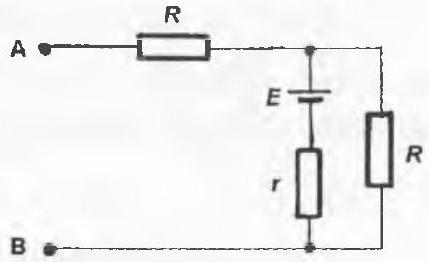
\includegraphics[max width=\textwidth, center]{2025_07_01_5b3ff9fa0d508c8e9f17g-169} Fig. 3.21\\

3.118.* Într-o bobinǎ cilindrică foarte lungă cu raza $r=6 \mathrm{~cm}$, având $n=8$ spire pe cm , străbatută de un curent $I=10 \mathrm{~A}$ se introduce un miez de fier moale cu $\mu_{r}=400$ şi lungimea $l_{1}=1,25 \mathrm{~cm}$. Fluxul magentic în bara de fier este:\\ A) $1 \mathrm{~Wb}$; B) $0,15 \mathrm{~Wb}$; C) $2,5 \mathrm{~Wb}$; D) $1,5 \mathrm{~Wb}$; E) $0,5 \mathrm{~Wb}$; F) $460 \mathrm{~mWb}$.\\ (Marcel Dobre)\\

3.119.* Ce frecvență are mişcarea de rotație a unui electron într-un loc unde componenta orizontală a câmpului magnetic terestru are valoarea $B=8 \pi \cdot 10^{-6} \mathrm{~T}$ ( $e=1,6 \cdot 10^{-19} \mathrm{C}, m_{0}=9,1 \cdot 10^{-31} \mathrm{~kg}$ ) ?\\ A) $3,2 \cdot 10^{7} \mathrm{~s}^{-1}$; B) $7,032 \cdot 10^{5} \mathrm{~s}^{-1}$; C) $8,12 \cdot 10^{5} \mathrm{~s}^{-1}$; D) $4,8 \cdot 106 \mathrm{~s}^{-1}$; E) $6,2 \cdot 10^{5} \mathrm{~s}^{-1}$; F) $9,11 \cdot 10^{7} \mathrm{~s}^{-1}$.\\ (Marcel Dobre)\\

3.120. Un aparat de prăjit pâinea are un rezistor din aliaj crom-nichel care funcționează la $120 \mathrm{~V}$. Când este pus în funcțiune la $0^{\circ} \mathrm{C}$, intensitatea curentului inițial care trece prin el este de $1,5 \mathrm{~A}$. Câteva secunde după aceea, intensitatea curentului atinge valoarea constantă $1,33 \mathrm{~A}$. Care este temperatura finală a rezistorului ? Valoarea medie a coeficientului termic al aliajului de crom-nichel pe intervalul respectiv de temperatură este de $0,45 \cdot 10^{-3} \mathrm{grad}^{-1}$.\\ A) $10^{\circ} \mathrm{C}$; B) $250 \mathrm{~K}$; C) $300^{\circ} \mathrm{C}$; D) $27^{\circ} \mathrm{C}$; E) $278^{\circ} \mathrm{C}$; F) $300 \mathrm{~K}$.\\ (Mădălina Puică)\\

3.121.* O bobină are 120 spire, lungimea $10 \pi \mathrm{~cm}$ şi este parcursă de un curent electric cu intensitatea de $1 \mathrm{~A}$. Ştiind că $\mu_{0}=4 \pi \cdot 10^{-7} \mathrm{H} / \mathrm{m}$, inducția magnetică în centrul bobinei este:\\ A) $4 \cdot 10^{-4} \mathrm{~T}$; B) $4,8 \cdot 10^{-4} \mathrm{~T}$; C) $5 \cdot 10^{-4} \mathrm{~T}$; D) $4,8 \mathrm{~T}$; E) $4,5 \cdot 10^{-4} \mathrm{~T}$; F) $8 \cdot 10^{-4} \mathrm{~T}$.\\ (Ion M. Popescu)\\

3.122.* O spiră în scurtcircuit, având rezistența $R=0,05 \Omega$, este parcursă de un flux magnetic $\Phi=10^{-5} \mathrm{~Wb}$ produs de un electromagnet. Întrerupând alimentarea electromagnetului, spira este parcursă de sarcina electrică:\\ A) $2 \mathrm{~C}$; B) $2 \cdot 10^{-3} \mathrm{C}$; C) $2 \cdot 10^{-4} \mathrm{C}$; D) $2,4 \cdot 10^{-4} \mathrm{C}$; E) $3 \cdot 10^{-4} \mathrm{C}$; F) $10^{-4} \mathrm{C}$.\\ (Ion M. Popescu)\\

3.123.* Traiectoria unui electron, a cărui sarcină specifică este $\frac{e}{m}=1,76 \cdot 10^{11} \mathrm{C} / \mathrm{kg}$, într-un câmp magnetic de inducție $B=7 \cdot 10^{-3} \mathrm{~T}$, este un arc de cerc cu raza $r=3 \mathrm{~cm}$. În acest caz, viteza $v$ a electronului este:\\ A) $3 \cdot 10^{7} \mathrm{~m} / \mathrm{s}$; B) $4 \cdot 10^{7} \mathrm{~m} / \mathrm{s}$; C) $3,7 \cdot 10^{7} \mathrm{~m} / \mathrm{s}$; D) $3,696 \cdot 10^{7} \mathrm{~m} / \mathrm{s}$; E) $3,5 \cdot 10^{7} \mathrm{~m} / \mathrm{s}$; F) $5 \cdot 10^{7} \mathrm{~m} / \mathrm{s}$.\\ (Ion M. Popescu)\\

3.124.* Un electron (cu $\frac{e}{m}=1,7 \cdot 10^{\mathrm{II}} \mathrm{C} / \mathrm{kg}$ ) care se mişcă în vid, într-un câmp magnetic de inducție $B=8 \cdot 10^{-3} \mathrm{~T}$, pe un cerc cu raza de $2 \mathrm{~cm}$, are viteza:\\ A) $2 \cdot 10^{7} \mathrm{~m} / \mathrm{s}$; B) $3 \cdot 10^{7} \mathrm{~m} / \mathrm{s}$; C) $2,7 \cdot 10^{7} \mathrm{~m} / \mathrm{s}$; D) $2,72 \cdot 10^{7} \mathrm{~m} / \mathrm{s}$; E) $2,6 \cdot 10^{7} \mathrm{~m} / \mathrm{s}$; F) $3,2 \cdot 10^{8} \mathrm{~m} / \mathrm{s}$.\\ (Ion M. Popescu)\\

3.125.* Pe lungimea $l$ a unei bobine fără miez sunt înfäşurate $N$ spire. Când prin bobină circulă un curent de intensitate $I$ fluxul magnetic în interior are o anumită valoare $\Phi$. Dacă se introduce în bobină un miez cu permeabilitatea relativă $\mu_{r}=128$, se reduce la jumătate numărul de spire (păstrând $l$ ) şi se reduce intensitatea curentului de 4 ori, fluxul devine $n \Phi$ unde $n$ este:\\ A) 256; B) 8; C) 64; D) 16; E) 6; F) 24.\\ (Constantin P. Cristescu)\\

3.126.* Un solenoid cu lungimea $l=0,2 \mathrm{~m}$ şi $N=250$ spire este parcurs de un curent electric cu intensitatea $I_{1}=0,4 \mathrm{~A}$. În interiorul său, în centru este plasată o spiră de rază $R=1 \mathrm{~cm}$ al cărei plan este paralel cu planul spirelor solenoidului. Intensitatea curentului care trebuie să circule prin spiră pentru ca inducția magnetică în centrul ei să fie nulă este:\\ A) $5,8 \mathrm{~A}$; B) $7 \mathrm{~A}$; C) $4,5 \mathrm{~A}$; D) $14 \mathrm{~A}$; E) $10 \mathrm{~A}$; F) $15 \mathrm{~A}$.\\ (Constantin P. Cristescu)\\

3.127.* Trei conductoare rectilinii paralele sunt situate într-un plan perpendicular pe planul foii. Cei trei curenți electrici au aceeaşi intensitate şi parcurg conductoarele în sensul arătat în Fig. 3.22. Forța care acționează asupra conductorului B este:\\ A) orientată perpendicular pe planul determinat de conductoare; B) orientată în sensul BC; C) orientată în sensul BA; D) nulă; E) orientată în lungul conductorului; F) nu se poate preciza din datele problemei.\\ (Constantin P. Cristescu)\\ 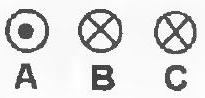
\includegraphics[max width=\textwidth, center]{2025_07_01_5b3ff9fa0d508c8e9f17g-171} Fig. 3.22\\

3.128.* O buclă dreptunghiulară cu dimensiunile $12 \mathrm{~cm} \times 18 \mathrm{~cm}$ se află lângă un fir rectiliniu, infinit lung. O latură a dreptunghiului este paralelă cu firul şi se află la distanta de $6 \mathrm{~cm}$, conform Fig. 3.23. Prin buclă circulă un curent de $60 \mathrm{~A}$, iar prin fir circulă un curent de $40 \mathrm{~A}$. Mărimea și direcția forței pe care o exercită firul asupra buclei este:\\ A) $9,8 \mathrm{~N}$ spre fir; B) $5,1 \cdot 10^{-3} \mathrm{~N}$ spre fir; C) $7,2 \cdot 10^{-4} \mathrm{~N}$ spre exterior; D) $7,2 \cdot 10^{-4} \mathrm{~N}$ spre fir; E) $1,2 \cdot 10^{5} \mathrm{~N}$ spre exterior; F) $1,2 \cdot 10^{5} \mathrm{~N}$ spre fir.\\ (Alexandrina Nenciu)\\ 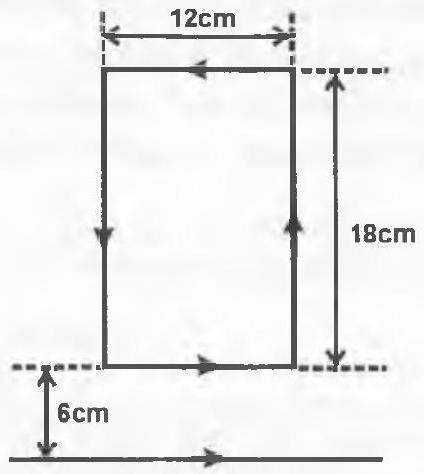
\includegraphics[max width=\textwidth, center]{2025_07_01_5b3ff9fa0d508c8e9f17g-171(1)} Fig. 3.23\\

3.129.* O buclă este formată din două semicercuri concentrice de raze $R$, respectiv $2 R$, conectate prin două segmente radiale (conform Fig. 3.24). Inducția magnetică $\vec{B}$ în centrul buclei este:\\ A) $B=\frac{\mu_{0} I}{8 R}$, iese din foaie; B) $B=\frac{\mu_{0} I}{4 R}$, intră în foaie; C) $B=\frac{\mu_{0} I}{8 R}$, intră în foaie; D) $B=\frac{\mu_{0} I}{R}$, intră în foaie; E) $B=\frac{3 \mu_{0} I}{4 R}$, iese din foaie; F) $B=\frac{\mu_{0} I}{2 R}$, iese din foaie.\\ (Alexandrina Nenciu)\\ 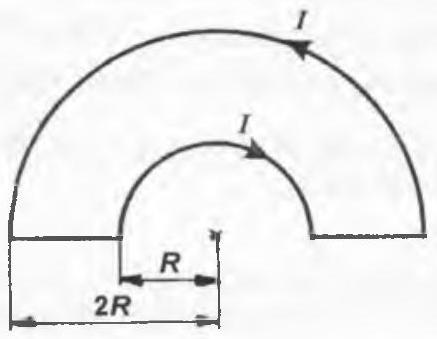
\includegraphics[max width=\textwidth, center]{2025_07_01_5b3ff9fa0d508c8e9f17g-171(2)} Fig. 3.24\\

3.130.* Un fir subțire, flexibil, prin care trece un curent de intensitate $I$ atârnă într-un câmp magnetic uniform, de inducție $\vec{B}$ conform Fig. 3.25. O greutate $\vec{G}$ este ataşată la unul din capetele firului, astfel că în fir apare tensiunea $T$. În câmp magnetic, porțiunea din fir se curbează şi ia forma unui arc de cerc. Raza cercului este:\\ A) $r=\frac{2 G}{B I}$; B) $r=\frac{G}{B I}$; C) $r=\frac{B I}{G}$; D) $r=\frac{2 B I}{G}$; E) $r=\frac{B I}{2 G}$; F) $r=\frac{G}{3 B I}$.\\ (Alexandrina Nenciu)\\ 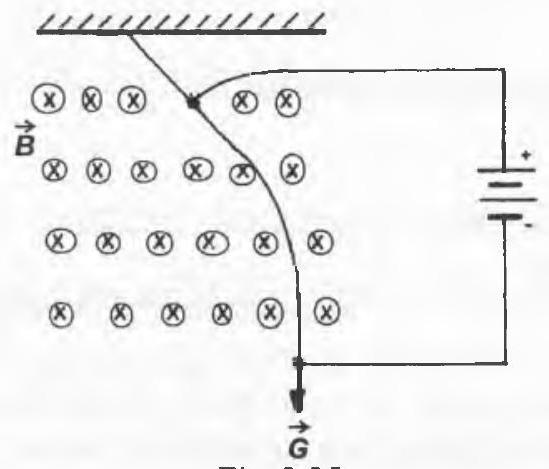
\includegraphics[max width=\textwidth, center]{2025_07_01_5b3ff9fa0d508c8e9f17g-172} Fig. 3.25\\

3.131.* Între polii unui electromagnet cu secțiunea $S=18 \mathrm{dm}^{2}$ se creează un flux magnetic $\Phi=0,45 \mathrm{~Wb}$. În acest spațiu se deplasează orizontal, sub acțiunea unei forțe mecanice constante $F=0,5 \mathrm{~N}$, un conductor având rezistența electrică $R=0,9 \Omega$ şi lungimea $l=30 \mathrm{~cm}$. Viteza limită (maximă) pe care o poate atinge conductorul pornind din repaus este egală cu :\\ A) $0,5 \mathrm{~m} / \mathrm{s}$; B) $0,8 \mathrm{~m} / \mathrm{s}$; C) $1 \mathrm{~m} / \mathrm{s}$; D) $2 \mathrm{~m} / \mathrm{s}$; E) $5 \mathrm{~m} / \mathrm{s}$; F) $9 \mathrm{~m} / \mathrm{s}$.\\ (Gabriela Cone)\\

3.132.* O tijă metalică se roteşte cu frecvența $n=600 \mathrm{rot} / \mathrm{min}$ în jurul unui ax care trece prin unul din capetele sale, în timp ce celălalt capăt alunecă pe un inel conductor de rază $r=10 \mathrm{~cm}$. Centrul inelului coincide cu axul de rotație al tijei Suprafața inelului este perpendiculară pe liniile unui câmp magnetic uniform de inducție $B=10^{-4} \mathrm{~T}$. Diferența de potențial indusă între capetele tijei este egală cu:\\ A) $1 \mathrm{~V}$; B) $3,14 \mathrm{mV}$; C) $31,4 \mu \mathrm{~V}$; D) $1 \mu \mathrm{~V}$; E) $1 \mathrm{~mV}$ ; F) $0,1 \mathrm{mV}$.\\ (Gabriela Cone)\\

3.133.* O particulă electrizată pătrunde cu viteza $v=200 \mathrm{~m} / \mathrm{s}$ într-un câmp magnetic uniform cu inducția $\bar{B}=1 \mathrm{~T}$, perpendicular pe liniile sale de câmp și descrie un sfert de cerc curaza $R=20,86 \mathrm{~cm}$. Durata mişcării particulei în câmp magnetic este :\\ A) $0,3 \mathrm{~s}$; B) $1,64 \mathrm{~ms}$; C) $0,58 \mathrm{~ms}$; D) $0,009 \mathrm{~s}$; E) $1 \mathrm{~s}$; F) $5 \mathrm{~s}$.\\ (Gabriela Cone)\\

3.134.* Un electron (de masă $m=9,1 \cdot 10^{-31} \mathrm{~kg}$ şi sarcină $q=1,6 \cdot 10^{-19} \mathrm{C}$ ) este accelerat de o sursă de tensiune şi atinge viteza $v=1,87 \cdot 10^{7} \mathrm{~m} / \mathrm{s}$. Cu această viteză, el intră într-o zonă cu câmp magnetic de inducție $B$ astfel dimensionat încât el să nu atingă un electrod aflat la distanța $d=1 \mathrm{~cm}$ de punctul în care a intrat în câmp. Viteza sarcinii şi inducția câmpului magnetic vor fi:\\ A) $v=2500 \mathrm{~km} / \mathrm{s} ; B=0,2 \mathrm{~T}$; B) $v=3400 \mathrm{~m} / \mathrm{s} ; B=2 \mathrm{~T}$; C) $v=1000 \mathrm{~km} / \mathrm{s} ; B=0,075 \mathrm{~T}$; D) $v=18700 \mathrm{~km} / \mathrm{s} ; B=1 / 100 \mathrm{~T}$; E) $v=18000 \mathrm{~cm} / \mathrm{s} ; B=1 / 5 \mathrm{~T}$; F) $v=25000 \mathrm{~km} / \mathrm{s} ; B=0,2 \mathrm{~T}$.\\ (Constantin Roşu)\\

3.135.* Două conductoare paralele, foarte lungi, sunt parcurse de curenții $I$ și $2 I$ în acelaşi sens. Valoarea maximă a forței care acționează pe unitatea de lungime a unui conductor paralel parcurs de curentul $3 I$, aflat într-un plan perpendicular pe planul conductoarelor, la mijlocul distanței $d$ dintre aceştia este:\\ A) $\frac{17 \mu I^{2}}{4 \sqrt{2} \pi d}$; B) $\frac{27 \mu I^{2}}{4 \sqrt{2} \pi d}$; C) $\frac{27 \mu I^{2}}{4 \pi d^{2}}$; D) $\frac{3 \mu I}{4 \sqrt{2} \pi d}$; E) $\frac{7 \mu I^{2}}{4 d}$; F) $\frac{27 \mu I^{2}}{3 \pi d^{2}}$.\\ (Constantin Roşu)\\

3.136.* Într-un cadru pătrat care se deplasează uniform într-un câmp magnetic paralel cu planul cadrului, avem:\\ A) intensitatea curentului variază sinusoidal; B) tensiunea indusă este nulă; C) curentul indus este maxim; D) curentul indus este constant şi diferit de zero; E) tensiunea indusă scade exponențial; F) debitul volumic este minim.\\ (Constantin Roşu)\\

3.137.* Două conductoare rectilinii, paralele, foarte lungi, sunt parcurse de curenți de intensități $1 \mathrm{~A}$ şi respectiv $2 \mathrm{~A}$ . Între conductoare se exercită forța de atracție pe unitatea de lungime de $0,5 \mathrm{~N} / \mathrm{m}$. Într-un punct din planul conductoarelor situat la distanță egală de conductoare, inducția magnetică este :\\ A) $0,1 \mathrm{~T}$; B) $0,5 \mathrm{~T}$; C) $1 \mathrm{~T}$; D) $1,5 \mathrm{~T}$; E) $2 \mathrm{~T}$; F) $0,25 \mathrm{~T}$.\\ (Tatiana Pop)\\

3.138.* Un conductor liniar de lungime $l=0,6 \mathrm{~m}$ cu rezistența $r=1 \Omega$ se deplasează pe două bare conductoare paralele de rezistență neglijabilă, cu viteza $v=10 \mathrm{~m} / \mathrm{s}$, normal pe un câmp magnetic omogen de inducție $B=0,5 \mathrm{~T}$ perpendicular pe planul barelor. Barele sunt legate prin rezistoarele $R_{1}=3 \Omega$, respectiv $R_{2}=6 \Omega$. Curenții $I_{1}$ şi $I_{2}$ care trec prin $R_{1}$, respectiv $R_{2}$, şi puterea mecanică necesară deplasării conductorului mobil au valorile:\\ A) $I_{1}=0,05 \mathrm{~A}, I_{2}=1 \mathrm{~A}, P=4,5 \mathrm{~W}$; B) $I_{1}=0,66 \mathrm{~A}, I_{2}=0,33 \mathrm{~A}, P=3 \mathrm{~W}$; C) $I_{1}=0,33 \mathrm{~A}, I_{2}=0,66 \mathrm{~A}, P=3 \mathrm{~W}$; D) $I_{1}=1 \mathrm{~A}, I_{2}=2 \mathrm{~A}, P=4,5 \mathrm{~W}$; E) $I_{1}=1 \mathrm{~A}, I_{2}=2 \mathrm{~A}, P=9 \mathrm{~W}$; F) $I_{1}=1 \mathrm{~A}, I_{2}=0,05 \mathrm{~A}, P=3 \mathrm{~W}$.\\ (Tatiana Pop)\\

3.139.* Un ion se deplasează cu viteza $v_{0}=2 \cdot 10^{6} \mathrm{~m} / \mathrm{s}$ într-un câmp magnetic uniform de inducție $B=0,4 \mathrm{~T}$, viteza ionului fiind perpendiculară pe liniile de câmp. Dacă raza traiectoriei descrisă de ion este $r=10,4 \mathrm{~cm}$, sarcina specifică a ionului are valoarea:\\ A) $2,08 \cdot 10^{6} \mathrm{C} / \mathrm{kg}$; B) $4,8 \cdot 10^{7} \mathrm{C} / \mathrm{kg}$; C) $3,2 \cdot 10^{6} \mathrm{C} / \mathrm{kg}$; D) $1,85 \cdot 10^{4} \mathrm{C} / \mathrm{kg}$; E) $1,85 \cdot 10^{-3} \mathrm{C} / \mathrm{kg}$; F) $1,76 \cdot 10^{8} \mathrm{C} / \mathrm{kg}$.\\ (Corneliu Ghizdeanu)\\

3.140.* Prin scoaterea miezului de fier având permeabilitatea relativă $\mu_{r}$, energia câmpului magnetic în interiorul unui solenoid parcurs de un curent electric constant se modifică în modul următor:\\ A) creşte de 2 ori; B) scade de 2 ori; C) creşte de $\mu_{r}$ ori; D) scade de $\mu_{r}$ ori; E) scade de $\left(\mu_{r} I\right)$ ori; F) creşte de ( $\mu_{r}-1$ ) ori.\\ (Corneliu Ghizdeanu)\\

3.141.* În atomul de hidrogen, electronul ( $q \equiv e$ ) se rotește în jurul nucleului pe o orbită circulară de rază $r_{0}$, cu viteza $v_{0}$, producând în centrul spirei o inducție magnetică:\\ A) $\frac{\mu_{0} e v_{0}}{\pi r_{0}}$; B) $\frac{2 \pi \mu_{0} e v_{0}}{r_{0}^{2}}$; C) $\mu_{0} \frac{e v_{0}}{r_{0}}$; D) $\mu_{0} \frac{e v_{0}}{4 \pi r_{0}^{2}}$; E) $\mu_{0} \frac{e v_{0}}{2 r_{0}^{2}}$; F) $\frac{\mu_{0} e v_{0}}{2 \pi}$.\\ (Corneliu Ghizdeanu)\\

3.142.* Prin trei conductoare rectilinii, lungi, paralele, plasate în vid la distanțe egale cu $d=6 \mathrm{~cm}$ unul de altul, trec curenții $I_{1}=I_{2}=-I_{3}=1 \mathrm{~A}$. Inducția magnetică într-un punct aflat la distanță egală de cele trei conductoare este:\\ A) $4,5 \mathrm{mT}$; B) $14,23 \mu \mathrm{~T}$; C) $2,35 \mathrm{mT}$; D) $11,53 \mu \mathrm{~T}$; E) $72,3 \mu \mathrm{~T}$; F) $3,5 \mu \mathrm{~T}$.\\ (Elena Slavnicu)\\

3.143.* O spiră circulară cu diametrul $d=16 \mathrm{~cm}$ se află într-un plan vertical, fiind aşezată perpendicular pe liniile unui câmp magnetic de inducție $B=10 \mathrm{mT}$. Spira este rotită cu un unghi egal cu $\frac{\pi}{6}$. Sarcina totală indusă în spiră dacă rezistența totală a bobinei galvanometrului înseriat cu ea este $R=2,5 \Omega$ va fi:\\ A) $36,19 \mu \mathrm{C}$; B) $17,26 \mu \mathrm{C}$; C) $10,77 \mu \mathrm{C}$; D) $18,38 \mu \mathrm{C}$; E) $12,39 \mu \mathrm{C}$; F) $15,77 \mu \mathrm{C}$.\\ (Elena Slavnicu)\\

3.144.* Energia înmagazinată în câmpul magnetic al unei bobine, dacă lungimea ei se dublează şi se introduce în interior un miez de fier cu permeabilitatea magnetică relativă $\mu_{r}=100$, se modifică în modul următor:\\ A) creşte de 100 ori; B) scade de 100 ori; C) creşte de 2 ori; D) scade de 2 ori; E) creşte de 50 ori; F) scade de 50 ori.\\ (Maria Honciuc)\\

3.145.* În circuitul din Fig. 3.26., bara AB se mişcă paralel cu ea însăşi de la vârful O spre dreapta, cu viteza $v=5 \mathrm{~m} / \mathrm{s}$ de-a lungul bisectoarei unghiului $\alpha$. Circuitul este plasat într-un câmp magnetic de inducție $B=1,5 \mathrm{~T}$ perpendicular pe planul circuitului. Rezistența unității de lungime a circuitului este $r=0,1 \Omega \cdot \mathrm{~m}^{-1}$ şi $\alpha=60^{\circ}$. Valoarea intensității curentului electric care ia naştere in circuit prin deplasarea barei AB este:\\ A) $15 \mathrm{~A}$; B) $25 \mathrm{~A}$; C) $10 \mathrm{~A}$; D) $5 \mathrm{~A}$; E) $30 \mathrm{~A}$; F) $20 \mathrm{~A}$.\\ (Maria Honciuc)\\ 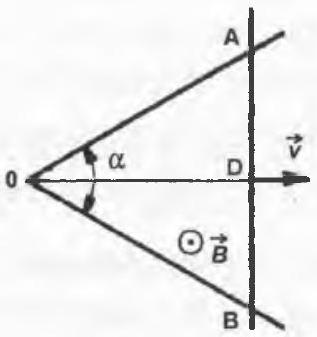
\includegraphics[max width=\textwidth, center]{2025_07_01_5b3ff9fa0d508c8e9f17g-175} Fig. 3.26\\

3.146.* Un electron se mişcă pe o traiectorie perpendiculară pe un câmp magnetic uniform. Dacă energia cinetică se dublează, frecvența de rotație creşte de:\\ A) de 2 ori; B) de $1 / 2$ ori; C) de 4 ori; D) nu se modifică; E) de $1 / 4$ ori; F) 7 ori.\\ (Cristina Stan)\\

3.147.* O bobină cu $N=2000$ spire dispuse pe o lungime $l=2 \mathrm{~cm}$, nu conține miez magnetic $\left(\mu_{0}=4 \pi \cdot 10^{-7} \mathrm{H} / \mathrm{m}\right)$ şi este străbătută de un curent $I=0,1 \mathrm{~A}$. Se plasează în centrul bobinei o spiră circulară, cu diametrul $D=1 \mathrm{~cm}$, perpendiculară pe liniile câmpului magnetic uniform creat de bobină. Știind că rezistența spirei este $R=20 \Omega$, iar $\pi^{2} \cong 10$, sarcina electrică totală care parcurge spira în timpul inversării sensului curentului electric prin bobină este:\\ A) $1 \mu \mathrm{C}$; B) nu se poate calcula pentru că nu se cunoaşte durata $\Delta t$ a inversării sensului curentului; C) $1 \mathrm{~mC}$; D) $0,1 \mu \mathrm{C}$; E) $0,5 \mu \mathrm{C}$; F) $0,5 \mathrm{C}$.\\ (Rodica Bena)\\

3.148.* Într-o spiră care se deplasează cu viteză constantă într-un câmp magnetic astfel încât liniile de câmp sunt mereu perpendiculare pe suprafața spirei:\\ A) tensiunea electromotoare indusă este maximă; B) curentul indus este alternativ; C) curentul indus este nul; D) curentul indus este constant; E) curentul indus este maxim; F) apare un curent autoindus constant.\\ (Rodica Bena)\\

3.149.* Într-un câmp magnetic de inducție $B=0,5 \mathrm{~T}$ pătrunde un ion pozitiv cu $v=10^{6} \mathrm{~m} / \mathrm{s}$, perpendicular pe direcția lui $\bar{B}$. Știind că raza traiectoriei descrise de ion în câmpul magnetic este $R=10 \mathrm{~cm}$, să se afle sarcina specifică.\\ A) $2 \cdot 10^{7} \mathrm{C} / \mathrm{kg}$; B) $5 \cdot 10^{-8} \mathrm{~kg} / \mathrm{C}$; C) $2 \cdot 10^{7} \mathrm{~kg} / \mathrm{C}$; D) $2 \cdot 10^{5} \mathrm{C} / \mathrm{kg}$; E) $5 \cdot 10^{-6} \mathrm{~kg} / \mathrm{C}$; F) $5 \cdot 10^{-8} \mathrm{C} / \mathrm{kg}$.\\ (Mona Mihăilescu)\\

3.150.* Două conductoare rectilinii, paralele şi foarte lungi, aşezate în aer ( $\mu=\mu_{0} \cong 4 \pi \cdot 10^{-7} \mathrm{~N} / \mathrm{A}^{2}$ ) la distanța $a=10 \mathrm{~cm}$ unul de altul, sunt parcurse de curenți având aceeaşi intensitate $I=30 \mathrm{~A}$, dar de sens contrar. Inducția câmpului magnetic în punctul situat la mijlocul distanței dintre ele este:\\ A) $5 \mathrm{~T}$; B) $3,5 \mathrm{~T}$; C) $4 \mathrm{~T}$; D) $2,4 \cdot 10^{-4} \mathrm{~T}$; E) $6,5 \cdot 10^{-3} \mathrm{~T}$; F) $7,5 \cdot 10^{-4} \mathrm{~T}$.\\ (Ion Belciu)\\

3.151.* O particulă încărcată electric, aflată în mişcare, pătrunde într-un câmp magnetic constant, după o direcție perpendiculară pe inducția câmpului $\vec{B}$ şi parcurge o traiectorie circulară de rază $R_{1}=4 \mathrm{~cm}$. Dacă particula pătrunde în acelaşi mod într-un câmp magnetic care şi-a dublat valoarea, raza traiectoriei, va fi:\\ A) $5 \mathrm{~cm}$; B)  $8 \mathrm{~cm}$; C) $2,5 \mathrm{~cm}$; D) $2 \mathrm{~cm}$; E) $3 \mathrm{~cm}$; F) $6,5 \mathrm{~cm}$.\\ (Ion Belciu)\\

3.152.* Un conductor liniar mobil cu lungimea $l=1,2 \mathrm{~m}$ este legat prin două conductoare de o sursă cu tensiunea electromotoare $E=24 \mathrm{~V}$ şi rezistență internă $r=0,5 \Omega$. Conductorul mobil se deplasează cu viteza $v=12,5 \mathrm{~m} / \mathrm{s}$ într-un câmp magnetic de inducție $B=0,8 \mathrm{~T}$, orientat ca în Fig. 3.27. Rezistența exterioară a circuitului fiind $R=2,5 \Omega$, intensitatea curentului din circuit este:\\ A) $8 \mathrm{~A}$; B) $6 \mathrm{~A}$; C) $7 \mathrm{~A}$; D) $4 \mathrm{~A}$; E) $8,66 \mathrm{~A}$; F) $9 \mathrm{~A}$.\\ (Ion Belciu)\\ 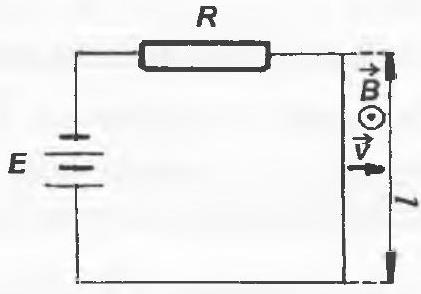
\includegraphics[max width=\textwidth, center]{2025_07_01_5b3ff9fa0d508c8e9f17g-177} Fig. 3.27\\

3.153.* O bară orizontală MN, perfect conductoare, de lungime $l=10 \mathrm{~cm}$ şi masă $m=100 \mathrm{~g}$ alunecă fară frecare de-a lungul a două bare perfect conductoare, plasate vertical și legate prin intermediul unui rezistor cu rezistența $R=0,1 \Omega$. Perpendicular pe planul barelor acționează un câmp magnetic omogen de inducție $B=1 \mathrm{~T}$. Lăsată să cadă sub efectul propriei greutăți de-a lungul celor două bare verticale ( $g=10 \mathrm{~m} / \mathrm{s}^{2}$ ), bara mobilă MN va atinge viteza limită:\\ A) $0,1 \mathrm{~ms}^{-1}$; B) $1 \mathrm{~ms}^{-1}$; C) $10 \mathrm{~ms}^{-1}$; D) $10^{-2} \mathrm{~ms}^{-1}$; E) $10^{-3} \mathrm{~ms}^{-1}$; F) $20 \mathrm{~ms}^{-1}$.\\ (Ilie Ivanov)\\

3.154.* Prin trei vârfuri ale unui pătrat cu latura $a=20 \mathrm{~cm}$ trec trei curenți perpendiculari pe planul pătratului având valorile: $I_{1}=100 \mathrm{~A}$ orientat în sens opus sensului celorlalți doi curenți alăturați, în dispunere consecutivă și cu valorile $I_{2}=2 I_{1}$ şi $I_{3}=I_{1}$. Inducția magnetică $\vec{B}$ produsă în vârful rămas liber va fi:\\ A) $2 \cdot 10^{-4} \mathrm{Wbm}^{-2}$; B) $2 \pi \cdot 10^{-4} \mathrm{Wbm}^{-2}$; C) $\frac{\pi}{2} \cdot 10^{-4} \mathrm{Wbm}^{-2}$; D) $4 \cdot 10^{-3} \mathrm{Wbm}^{-2}$; E) $2 \mathrm{Wbm}^{-2}$; F) $0,2 \mathrm{Wbm}^{-2}$.\\ (Ilie Ivanov)\\

3.155.* Un electron se mişcă pe o traiectorie circulară de rază $1,2 \mathrm{~cm}$, perpendiculară pe un câmp magnetic uniform. Viteza electronului este de $10^{6} \mathrm{~m} / \mathrm{s}$. Care este fluxul magnetic total care străbate orbita ?\\ A) $2,14 \cdot 10^{-4} \mathrm{~Wb}$; B) $2,14 \cdot 10^{-7} \mathrm{~Wb}$; C) $3,14 \cdot 10^{-7} \mathrm{Tm}^{2}$; D) $2,14 \cdot 10^{-7} \mathrm{mWb}$; E) $2,14 \cdot 10^{-7} \mathrm{mTm}^{2}$; F) $3,14 \cdot 10^{-7} \mathrm{Tcm}^{2}$.\\ (Mădălina Puică)\\

3.156.* Un fir rectiliniu lung este parcurs de un curent cu intensitatea de $1,5 \mathrm{~A}$. Un electron se deplasează cu o viteză de $5 \cdot 10^{6} \mathrm{~cm} / \mathrm{s}$ paralel cu firul, la $10 \mathrm{~cm}$ distantă, și în acelaşi sens cu curentul. Ce forță exercită câmpul magnetic al curentului asupra electronului în mişcare ?\\ A) $5 \mathrm{~mN}$; B) $10^{-4} \mathrm{~N}$; C) $2,4 \cdot 10^{-20} \mathrm{~N}$; D) $2,5 \mathrm{~N}$; E) $10^{-3} \mathrm{~N}$; F) $10^{-31} \mathrm{~N}$.\\ (Mădălina Puică)\\

3.157.* Un iluzionist amator vrea să arate familiei cum "pluteşte în aer" un fir de aluminiu, cu diametrul de $0,5 \mathrm{~mm}$ şi densitatea $\rho=2700 \mathrm{~kg} \cdot \mathrm{~m}^{-3}$, folosindu-se de un conductor liniar de cupru fixat de masă, paralel cu cel de aluminiu, prin care circulă un curent de $175 \mathrm{~A}$ . La ce distanță maximă deasupra mesei ar sta în echilibru conductorul de aluminiu, dacă prin el poate circula un curent maxim de $40 \mathrm{~u.S.I.}$, în sensul curentului din conductorul fix ?\\ A) $15 \mathrm{~mm}$ deasupra firului de cupru; B) $3,8 \mathrm{~mm}$ deasupra firului de cupru; C) demonstrația nu reuşeşte, firul de Al nu pluteşte; D) $3,8 \mathrm{~mm}$ lateral spre Nord; E) $15 \mathrm{~mm}$ lateral spre Vest; F) $7,5 \mathrm{~mm}$ deasupra.\\ (Radu Chişleag)\\

3.158.* Un conductor liniar, parcurs de un curent de $50 \mathrm{~A}$ , se află într-un câmp magnetic uniform exterior de inducție $B_{e}=1 \mathrm{mT}$, normal pe conductor. Care este locul geometric al punctelor în care câmpul magnetic local este nul ?\\ A) un plan care conține conductorul şi este paralel cu $\vec{B}_{e}$; B) un plan care conține conductorul și este perpendicular pe $\vec{B}_{e}$; C) un cilindru drept cu raza $r=10 \mathrm{~mm}$, centrat pe conductor; D) un trunchi de con cu vârful la mijlocul conductorului şi cu unghiul la vârf de $\pi / 2$; E) o dreaptă paralelă cu conductorul la distanța de $10 \mathrm{~mm}$ de acesta, aflată într-un plan perpendicular pe $\vec{B}_{e}$; F) un cerc aflat într-un plan perpendicular pe conductor, cu raza de $1 \mathrm{~cm}$.\\ (Radu Chişleag)\\

3.159.* Câmpului magnetic terestru $\vec{B}_{0}$ orientat spre Nord i se suprapune un câmp magnetic $\vec{B}$ uniform orientat spre Est, de intensitate $B=\sqrt{3} B_{0}$. Ce direcție va indica acul magnetic al unei busole plasate în planul vectorilor $\vec{B}$ şi $\vec{B}_{0}$ ?\\ A) Nord - Est, făcând un unghi de $30^{\circ} \mathrm{C}$ cu direcția Est; B) Nord - Est, fåcând un unghi de $30^{\circ}$ cu direcţia Nord; C) Nord - Est, făcând un unghi de $\pi / 3$ cu direcția Nord; D) Sud - Vest, făcând un unghi de $45^{\circ}$ cu direcția Sud; E) Sud - Vest, făcând un unghi de $30^{\circ}$ cu direcția Vest; F) Nord - (Nord - Est).\\ (Radu Chişleag)\\

3.160.* Un solenoid având $8$ spire/$\mathrm{cm}$, foarte lung, este parcurs de un curent cu intensitatea de $16 \mathrm{~A}$ . Pe axul solenoidului este plasat un conductor având lungimea de $25 \mathrm{~cm}$ , prin care circulă acelaşi curent ca şi prin solenoid. Care este forța exercitată de solenoid asupra conductorului axial ?\\ A) $0,01 \mathrm{~N}$ în sensul curentului; B) $0,04 \mathrm{~N}$ în sensul curentului; C) $0,01 \mathrm{~N}$ în sensul opus curentului; D) $0,04 \mathrm{~N}$ în sensul opus curentului; E) 0; F) Forța nu se poate determina cantitativ deoarece ångstromul nu este o unitate pentru intensitatea curentului electric.\\ (Radu Chişleag)\\

3.161.* Un solenoid cu lungimea $l$ și fără miez magnetic are inductanța $L_{0}=0,24 \mathrm{H}$. În solenoid se introduce un miez de lungimea solenoidului format din doi cilindri de materiale feromagnetice, unul de lungime $0,8 l$ şi permeabilitate relativă 750, iar celălalt pe restul lungimii, de permeabilitate relativă 250 . Care este inductanța noului solenoid ?\\ A) $84 \mathrm{~H}$; B) $0,65 \mathrm{H}$; C) $0,89 \mathrm{H}$; D) $240 \mathrm{~H}$; E) $156 \mathrm{~H}$; F) $1200 \mathrm{~mH}$.\\ (Radu Chişleag)\\

3.162.* Tensiunea la bornele unei surse de curent continuu $U_{B}$ este mai mare decât tensiunea ei electromotoare $E$ dacă sursa considerată este legată:\\ A) în serie cu un rezistor având rezistența infinită; B) în paralel cu o altă sursă având $E^{\prime}>E$; C) în serie cu o altă sursă având $E^{\prime}>E$; D) în opoziție cu o altă sursă având $E^{\prime}>E$; E) în serie cu o altă sursă având $E^{\prime}<E$; F) nu se poate obține o asmenea situație.\\ (Nicoleta Eşeanu)\\

3.163.* Alegeți varianta corectă pentru orientarea forței Lorentz (pentru cazurile A, C şi E sarcina electrică este pozitivă, iar pentru celelalte sarcina electrică este negativă; Fig. 3.28):\\ A) 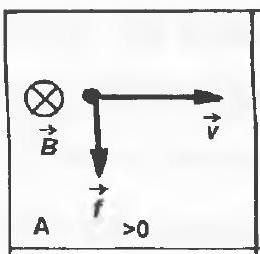
\includegraphics[max width=\textwidth, center]{2025_07_01_5b3ff9fa0d508c8e9f17g-180(1)A}; B) 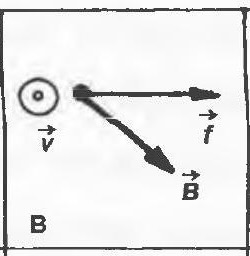
\includegraphics[max width=\textwidth, center]{2025_07_01_5b3ff9fa0d508c8e9f17g-180(1)B}; C) 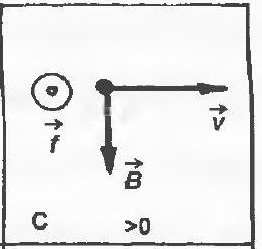
\includegraphics[max width=\textwidth, center]{2025_07_01_5b3ff9fa0d508c8e9f17g-180(1)C}; D) 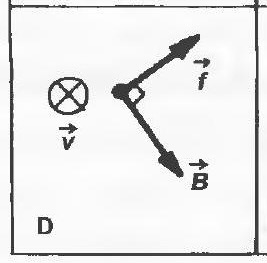
\includegraphics[max width=\textwidth, center]{2025_07_01_5b3ff9fa0d508c8e9f17g-180(1)D}; E) 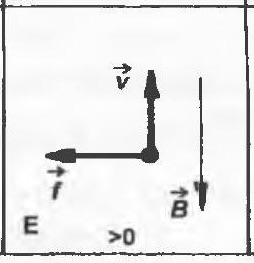
\includegraphics[max width=\textwidth, center]{2025_07_01_5b3ff9fa0d508c8e9f17g-180(1)E}; F) 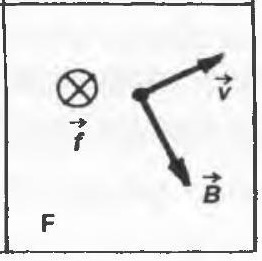
\includegraphics[max width=\textwidth, center]{2025_07_01_5b3ff9fa0d508c8e9f17g-180(1)F}.\\ (Nicoleta Eşeanu)\\ 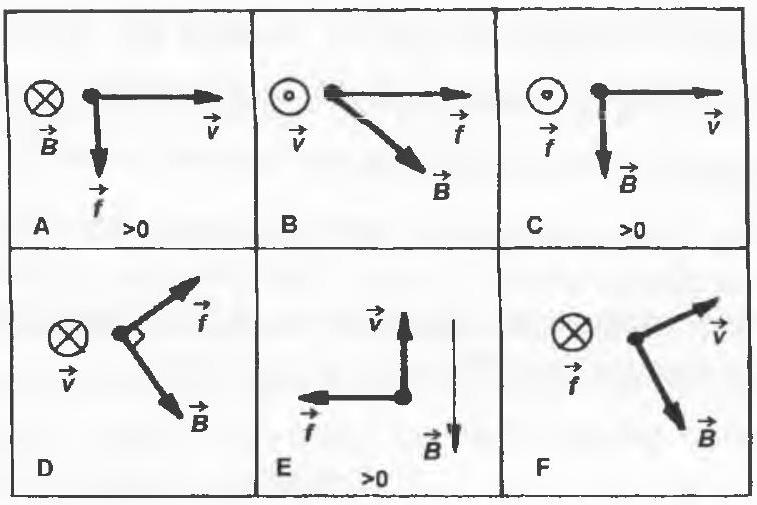
\includegraphics[max width=\textwidth, center]{2025_07_01_5b3ff9fa0d508c8e9f17g-180(1)} Fig. 3.28\\

3.164.* Alegeți afirmația corectă referitoare la fenomenul de inducție electromagnetică:\\ A) tensiunea electromotoareindusă într-un circuit depinde numai de aria circuitului şi de inducția magnetică; B) tensiunea electromotoareindusă într-un circuit este egală cu fluxul magnetic prin suprafața acelui circuit luat cu semn schimbat; C) tensiunea electromotoareindusă într-o bobină cu $N$ spire este de $N$ ori mai mică decât cea indusă într-o spiră; D) tensiunea electromotoareindusă într-un circuit este egală cu viteza de variație a fluxului magnetic prin suprafața acelui circuit luată cu semn schimbat; E) sensul curentului indus este astfel încât fluxul său magnetic se opune fluxului magnetic inductor; F) nici o variantă din cele anterioare nu este corectă.\\ (Nicoleta Eşeanu)\\

3.165.* În montajul din Fig. 3.29 se cunosc: $R=2 \mathrm{k} \Omega, R_{b}=8 \mathrm{k} \Omega, L=12 \mathrm{mH}$ şi $U=200 \mathrm{~V}$. Fluxul magnetic în bobină este:\\ A) $6 \cdot 10^{-5} \mathrm{~Wb}$; B) $12 \mathrm{~mWb}$; C) $0,1 \mathrm{~Wb}$; D) $0,24 \mathrm{mWb}$; E) $0,84 \mathrm{~Wb}$; F) $0,2 \mathrm{mT}$.\\ (Nicoleta Eşeanu)\\ 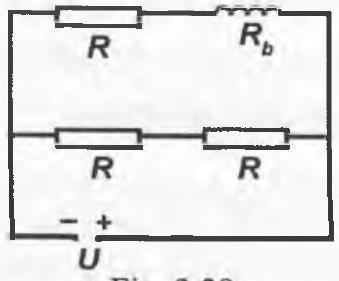
\includegraphics[max width=\textwidth, center]{2025_07_01_5b3ff9fa0d508c8e9f17g-180} Fig. 3.29\\

3.166.* Prin vârfurile $\mathrm{A}, \mathrm{B}, \mathrm{C}$ şi $\mathrm{D}$ ale unui pătrat de latură $a$ trec patru conductoare paralele, infinit de lungi, perpendiculare pe planul pătratului, străbătute, în ordine, de următorii curenți: $I_{1}=2 I, I_{2}=I_{3}=I_{4}=I$. Curenții $I_{1}$ şi $I_{2}$ au sensul dinspre observator spre planul foii, iar ceilalți au sens invers față de primii doi. Forța pe unitatea de lungime care se exercită asupra conductorului $I_{3}$ este:\\ A) $\frac{\mu I^{2}(2+\sqrt{2})}{2 \pi a}$; B) $\frac{\mu I^{2}(2-\sqrt{2})}{2 \pi a}$; C) $\frac{2 \mu I^{2}}{\pi a}$; D) $\frac{\mu I^{2}}{\pi a}$; E) $\frac{2 \mu I^{2}(1+\sqrt{2})}{\pi a}$; F) nici o variantǎ nu este corectă.\\ (Nicoleta Eşeanu)\\

3.167.* O particulă având sarcina $q=3,2 \cdot 10^{-19} \mathrm{C}$ şi masa $m=1,7 \cdot 10^{-27}$ kg descrie un cerc de rază $r=2 \mathrm{~cm}$ într-un câmp magnetic uniform de inducție $B=27 \mathrm{mT}$. Viteza particulei este:\\ A) $101 \mathrm{~km} / \mathrm{s}$; B) $7,8 \cdot 10^{-3} \mathrm{~m} / \mathrm{s}$; C) $1,25 \cdot 10^{7} \mathrm{~m} / \mathrm{s}$; D) $640 \mathrm{~m} / \mathrm{s}$; E) $160 \mathrm{~m} / \mathrm{s}$; F) $228 \mathrm{~m} / \mathrm{s}$.\\ (Nicoleta Eşeanu)\\

3.168.* O bobină cu $n=10$ spire $/ \mathrm{cm}$ are volumul interior $V=10 \pi \mathrm{~cm}^{3}$ ocupat de un miez magnetic având permeabilitatea relativă $\mu_{r}=380$. Cunoaştem $\mu_{0}=4 \pi \cdot 10^{-7} \mathrm{~N} / \mathrm{A}^{2}$ şi $\pi^{2} \approx 10$. Inductanţa bobinei este:\\ A) $7,8 \mathrm{mH}$; B) $0,03 \mathrm{H}$; C) $3,8 \mathrm{mH}$; D) $15,2 \mathrm{mH}$; E) $4 \pi^{2} \cdot 10^{-3} \mathrm{H}$; F) $4 \pi \cdot 10^{-3} \mathrm{H}$.\\ (Nicoleta Eşeanu)\\

3.169.* Un solenoid cu lungimea $\ell=0,5 \mathrm{~m}$ şi cu $n=200$ spire $/ \mathrm{m}$ este parcurs de un curent de intensitate $I=1 \mathrm{~A}$. Firul conductor (subțire) este înfăşurat pe un miez având aria secțiunii transversale $S=20 \mathrm{~cm}^{2}$ şi permeabilitatea relativă $\mu_{r}=400$. Intrerupem curentul într-un interval de timp $\Delta t=0,02 \mathrm{~s}$. Diferența de potențial apărută la bornele solenoidului este:\\ A) $(6,4 \pi) \mathrm{mV}$; B) $5,4 \mathrm{mV}$; C) $(0,32 \pi) \mathrm{V}$; D) $(8 \pi) \mathrm{V}$; E) $(0,4 \pi) \mathrm{mV}$; F) nici o variantă nu este corectă.\\ (Nicoleta Eşeanu)\\

3.170.* Un contur metalic pătrat, de latură $a=10 \mathrm{~cm}$ şi rezistență $R=2 \Omega$, este aşezat pe un plan orizontal într-un loc unde componenta verticală a câmpului magnetic terestru este $B_{v}=50 \mu \mathrm{~T}$. Răsturnăm conturul cu $180^{\circ}$ într-un interval de timp de $3 \mathrm{~s}$. Sarcina electrică ce trece prin cadru este:\\ A) $0,15 \mathrm{mC}$; B) $250 \mathrm{~nC}$; C) $13,33 \mu \mathrm{C}$; D) $0,5 \mu \mathrm{C}$; E) $0,85 \mathrm{mC}$; F) $0,35 \mathrm{mC}$.\\ (Nicoleta Eşeanu)\\

3.171.* Un electron şi o particulă $\alpha$ se mişcă într-un câmp magnetic pe traiectorii circulare cu aceeaşi viteză. Raportul dintre numărul de rotații pe secundă pe care le efectuează electronul şi respectiv particula $\alpha$ este egal cu (se dau: $m_{e}=9,1 \cdot 10^{-31} \mathrm{~kg}, m_{\alpha}=6,68 \cdot 10^{-27} \mathrm{~kg}$ şi sarcina particulei $q_{\alpha}=2 e$, unde $e$ este sarcina electronului):\\ A) 367; B) 4000; C) 36,7; D) 3670,3; E) 6703; F) 1813.\\ (Răzvan Mitroi)\\

3.172.* Un solenoid cu lungimea de $30 \mathrm{~cm}$ este bobinat cu două straturi de sârmă. Stratul interior conține 300 spire, iar cel exterior 250 spire. Curentul care trece prin solenoid are intensitatea de $3 \mathrm{~A}$ şi circulă în acelaşi sens în ambele straturi. Inducția magnetică într-un punct din apropierea axei solenoidului are valoarea:\\ A) $10^{-3} \mathrm{~T}$; B) $6,9 \cdot 10^{-3} \mathrm{~A}$; C) $690 \mathrm{~T}$; D) $9 \cdot 10^{-3} \mathrm{~T}$; E) $\left.6,9 \cdot 10^{-3} \mathrm{~T}$; F) $0,9 \mathrm{~T}$.\\ (Răzvan Mitroi)\\

3.173.* Într-un câmp magnetic de inducție $B=0,4 \mathrm{~T}$ este plasată o bobină cu $N=300$ spire, având rezistența spirelor $R=40 \Omega$ şi aria secțiunii transversale $S=16 \mathrm{~cm}^{2}$. Bobina este astfel plasată încât axa sa face un unghi $\alpha=60^{\circ}$ cu direcția câmpului magnetic. Sarcina electrică ce trece prin bobină dacă câmpul magnetic se întrerupe brusc este egală cu:\\ A) $2,4 \cdot 10^{-3} \mathrm{~A}$; B) $4 \cdot 10^{-3} \mathrm{C}$; C) $7,4 \cdot 10^{-3} \mathrm{C}$; D) $2,4 \cdot 10^{-3} \mathrm{C}$; E) $24 \cdot 10^{-3} \mathrm{C}$; F) $2 \cdot 10^{-3} \mathrm{~A}$.\\ (Răzvan Mitroi)\\

3.174.* O spiră aflată în scurtcircuit, având rezistența $R=0,1 \Omega$ este parcursă de un flux magnetic $\Phi$ produs de un electromagnet. Sarcina electrică totală care parcurge spira dacă se întrerupe alimentarea electromagnetului are valoarea de $10^{-3} \mathrm{C}$. Fluxul magnetic produs de electromagnet este egal cu:\\ A) $5 \cdot 10^{-2} \mathrm{~Wb}$; B) $2 \cdot 10^{-3} \mathrm{~Wb}$; C) $5 \cdot 10^{-4} \mathrm{~Wb}$; D) $10^{-4} \mathrm{~Wb}$; E) $10^{-5} \mathrm{~Wb}$; F) $10^{-3} \mathrm{~Wb}$.\\ (Ileana Creangă)\\

3.175.* În interiorul unui solenoid cu lungimea $l=0,25 \mathrm{~m}$ și numărul de spire $N=300$, aflat în aer, se găseşte un inel metalic de arie $S=5 \cdot 10^{-4} \mathrm{~m}^{2}$ şi rezistență $R=0,02 \Omega$. Suprafața inelului este perpendiculară pe axa solenoidului. Curentul în solenoid variază după legea $I=k t$, unde $k=1 \mathrm{~A} / \mathrm{s}$. Forța pe unitatea de lungime care acționează asupra inelului după $5 \mathrm{~s}$ de la închiderea circuitului este:\\ A) $7,1 \mathrm{~N} / \mathrm{m}$; B) $28,4 \cdot 10^{-8} \mathrm{~N} / \mathrm{m}$; C) $7,1 \cdot 10^{-5} \mathrm{~N} / \mathrm{m}$; D) $10^{-8} \mathrm{~N}$; E) $51000 \mathrm{~N} / \mathrm{m}$; F) $10^{-6} \mathrm{~N} / \mathrm{m}$.\\ (Ileana Creangă)\\

3.176.* O tijă metalică (Fig. 3.30) de masă $m=0,1 \mathrm{~kg}$ şi lungimea $25 \mathrm{~cm}$ cade de-a lungul unor şine verticale considerate fără rezistență electrică. În regiunea şinelor acționează un câmp magnetic omogen cu inducția $2 \mathrm{~T}$ , normal pe planul şinelor. Şinele verticale sunt legate între ele cu un rezistor de $1 \Omega$. Se neglijează frecările. Se dă $g=10 \mathrm{~m} / \mathrm{s}^{2}$. Viteza limită de cădere a tijei este:\\ A) $1 \mathrm{~m} / \mathrm{s}$; B) $10 \mathrm{~m} / \mathrm{s}$; C) $4 \mathrm{~m} / \mathrm{s}$; D) $50 \mathrm{~m} / \mathrm{s}$; E) $0,1 \mathrm{~m} / \mathrm{s}$; F) $8 \mathrm{~m} / \mathrm{s}$.\\ (Niculae Puşcaş)\\ 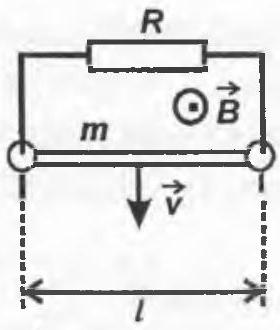
\includegraphics[max width=\textwidth, center]{2025_07_01_5b3ff9fa0d508c8e9f17g-183} Fig. 3.30\\

3.177.* O bară metalică de lungime $1 \mathrm{~m}$ şi masă $2 \mathrm{~kg}$ se mişcă fără frecare pe o masă orizontală. De mijlocul barei este legat un fir fără greutate care este trecut apoi peste un scripete ideal, fixat la marginea mesei, la celălalt capăt al firului fiind suspendat un corp de $1 \mathrm{~kg}$. Mişcarea barei are loc într-un câmp magnetic cu inducția $2 \cdot 10^{-4} \mathrm{~T}$. Diferența de potențial de la capetele barei după $3 \mathrm{~s}$ de la începutul mişcării sale este ( $g=10 \mathrm{~m} / \mathrm{s}^{2}$ ):\\ A) $1 \mathrm{~V}$; B) $0,2 \mathrm{~V}$; C) $10 \mathrm{~V}$; D) $0,01 \mathrm{~V}$; E) $2 \cdot 10^{-3} \mathrm{~V}$; F) $8 \mathrm{~mV}$.\\ (Niculae Puşcaş)\\

3.178.* Între două conductoare verticale, paralele, fixe, presupuse infinit de lungi, parcurse de curenți cu intensitatea de $1 \mathrm{~A}$, respectiv $2 \mathrm{~A}$, în acelaşi sens, se suspendă un al treilea conductor, paralel cu primele, la distanţa de $0,05 \mathrm{~m}$ faţă de primul conductor. Distanța dintre primele două conductoare astfel încât al treilea conductor, care se poate deplasa lateral în planul celorlalte două, să fie în echilibru, este:\\ A) $1 \mathrm{~m}$; B) $0,5 \mathrm{~m}$; C) $0,15 \mathrm{~m}$; D) $0,01 \mathrm{~m}$; E) $10^{-3} \mathrm{~m}$; F) $0,75 \mathrm{~m}$.\\ (Niculae Puşcaş)\\

3.179.* Din două conductoare identice de lungime $L$ se formează o spiră circulară şi una sub formă de triunghi echilateral. Aceste spire sunt traversate perpendicular de liniile unui câmp magnetic variabil $B=B(t)$. Raportul între curentul indus în spira circulară şi cel indus în spira triunghiulară este:\\ A) $\frac{3 \sqrt{3}}{\pi}$; B) $\frac{\pi \sqrt{3}}{2}$; C) $\frac{3 \sqrt{2}}{\pi}$; D) $\frac{2 \sqrt{3}}{\pi}$; E) $\frac{2 \pi}{\sqrt{3}}$; F) $\frac{3 \pi}{\sqrt{2}}$.\\ (Mihai Cristea)\\

3.180.* Un electron (de sarcină $e=1,6 \cdot 10^{-19} \mathrm{C}$ ) este accelerat într-o tensiune $U=20 \mathrm{~V}$ și intră apoi perpendicular pe inducția unui câmp magnetic omogen. Dacă electronul descrie în jurul inducției un cerc de rază $r=0,5 \mathrm{~cm}$, forța Lorentz ce acționează asupra electronului este egală cu:\\ A) $3,2 \cdot 10^{-19} \mathrm{~N}$; B) $1,28 \cdot 10^{-15} \mathrm{~N}$; C) $4,18 \cdot 10^{-16} \mathrm{~N}$; D) $8 \cdot 10^{-19} \mathrm{~N}$; E) $5,4 \cdot 10^{-18} \mathrm{~N}$; F) $2,8 \cdot 10^{-17} \mathrm{~N}$.\\ (Mircea Stan)\\

3.181.* Inducția magnetică în centrul unei bobine cu 50 spire, lungime $5 \mathrm{~cm}$ , parcurse de un curent electric cu intensitatea de $1,5 \mathrm{~A}$, dacă bobina are un miez de fier cu $\mu_{r}=200\left(\mu_{0}=4 \pi \cdot 10^{-7} \mathrm{~N} / \mathrm{A}^{2}\right)$ are valoarea:\\ A) $25 \cdot 10^{-7} \mathrm{~T}$; B) $0,12 \pi \mathrm{~T}$; C) $20 \pi \cdot 10^{-5} \mathrm{~T}$; D) $30 \pi \mathrm{~T}$; E) $2,4 \pi \mathrm{~T}$; F) $50 \cdot 10^{-3} \mathrm{~T}$.\\ (Gabriela Tiriba)\\

3.182.* Două conductoare foarte lungi, paralele, aflate la distanța $d=12 \mathrm{~cm}$ unul de celălalt sunt parcurse de curenți de acelaşi sens având intensitățile $I_{1}=2 \mathrm{~A}$ şi $I_{2}=5 \mathrm{~A}$. Inducția magnetică a câmpului rezultant la jumătatea distanței dintre cele două conductoare $\left(\mu_{0}=4 \pi \cdot 10^{-7} \mathrm{~N} / \mathrm{A}^{2}\right)$ are valoarea:\\ A) $10^{-5} \mathrm{~T}$; B) $2 \cdot 10^{-7} \mathrm{~T}$; C) $3 \cdot 10^{-5} \mathrm{~T}$; D) $7 \cdot 10^{-7} \mathrm{~T}$; E) $12 \pi \cdot 10^{-7} \mathrm{~T}$; F) $1,5 \cdot 10^{-3} \mathrm{~T}$.\\ (Gabriela Tiriba)\\

3.183.* Un conductor rectiliniu, de lungime $l$, parcurs de un curent constant $I$, este plasat într-un câmp magnetic uniform, de inducție $\vec{B}$. Asupra acestuia va acționa forța electromagnetică $\vec{F}$. Care dintre afirmaţiile următoare este falsă?\\ A) forța $\vec{F}$ este perpendiculară pe inducția magnetică $\vec{B}$; B) valoarea forței $F$ este maximă când conductorul este perpendicular pe liniile de câmp magnetic; C) forța $\vec{F}$ este perpendiculară pe viteza de transport a electronilor prin conductor; D) valoarea forței $F$ este maximă când conductorul este paralel cu liniile de câmp magnetic; E) valoarea forței $F$ este proporțională cu numărul de electroni care străbat conductorul în unitatea de timp; F) toate afirmațiile anterioare sunt false.\\ (Eugen Scarlat)\\

3.184.* Ţinând cont de relația cu care se calculează mărimea forței electromagnetice ce acționează asupra unui conductor rectiliniu, $F=B I l \sin \alpha$, una dintre afirmațiile următoare este falsă:\\ A) $I$ este intensitatea curentului care trece prin conductor; B) $B$ este inducția magnetică a câmpului produs de curentul $I$; C) $\alpha$ este unghiul format de vectorul $\vec{B}$ cu directia conductorului; D) $l$ este lungimea porțiunii de conductor care se află în câmpul magnetic; E) forţa $\vec{F}$ este perpendiculară pe planul determinat de vectorul inducție magnetică şi de conductor; F) toate afirmațiile anterioare sunt false.\\ (Eugen Scarlat)\\

3.185.* Care dintre următoarele afirmații referitoare la forța Lorentz este falsă:\\ A) sensul forței Lorentz depinde de semnul sarcinii electrice asupra căreia acționează; B) valoarea forței Lorentz depinde de viteza sarcinii electrice; C) forța Lorentz modifică energia cinetică a particulei; D) forța Lorentz nu acționează asupra particulelor fară sarcină electrică; E) forța Lorentz modifică vectorul viteză a particulei; F) toate afirmațiile anterioare sunt false.\\ (Eugen Scarlat)\\

3.186.* O spiră conductoare plană este plasată într-un câmp magnetic crescător în timp. Care dintre afirmațiile următoare nu este adevărată?\\ A) fenomenul de inducție electromagnetică nu se poate pune în evidență în lipsa spirei conductoare; B) sensul câmpului magnetic indus este opus celui al câmpului magnetic inductor; C) valoarea tensiunii electromotoareinduse în spiră este proporțională cu suprafața spirei; D) valoarea tensiunii electromotoare induse în spiră este mai mare dacă intervalul de timp în care fluxul câmpului inductor are o variație dată este mai scurt; E) tensiunea electromotoare indusă în spiră este nulă dacă planul spirei este paralel cu liniile de câmp magnetic; F) toate afirmațiile anterioare sunt false.\\ (Eugen Scarlat)\\

3.187.* În relația care defineşte modulul forței Lorentz $f$ ce acționează asupra unei particule cu sarcina electrică $q$ si se mişcă cu viteza $v, f=q v B \sin \alpha$, una dintre afirmațiile următoare este falsă:\\ A) forța Lorentz $\vec{f}$ este perpendiculară pe vectorul inducție magnetică $\vec{B}$; B) forța Lorentz $\vec{f}$ este perpendiculară pe vectorul viteză $\vec{v}$ a particulei; C) unghiul $\alpha$ este unghiul dintre vectorul inducție magnetică $\vec{B}$ şi vectorul viteză a particulei $\vec{v}$; D) forța Lorentz modifică valoarea vitezei particulei; E) forța Lorentz este nulă dacă particula se mişcă în lungul liniilor de câmp magnetic; F) toate afirmațiile anterioare sunt false.\\ (Eugen Scarlat)\\

3.188.* Doi solenoizi identici $L_{A}$ şi $L_{B}$ sunt conectați în serie într-un circuit de curent continuu, prima dată ca în Fig. 3.31a, iar a doua oară ca în Fig. 3.31b, astfel ca sensurile de bobinaj ale celor doi solenoizi să fie contrare în cazul b). Inducția magnetică din centrul solenoidului $L_{\mathrm{A}}$ :\\ A) rămâne neschimbată; B) creşte de două ori; C) creşte de patru ori; D) scade de două ori; E) scade de patru ori; F) devine zero.\\ (Eugen Scarlat)\\ 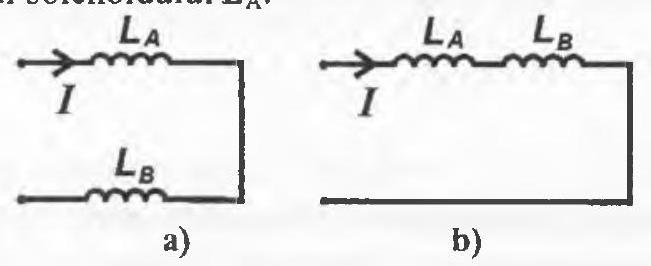
\includegraphics[max width=\textwidth, center]{2025_07_01_5b3ff9fa0d508c8e9f17g-187} Fig. 3.31\\

3.189.* Doi solenoizi identici $L_{\mathrm{A}}$ şi $L_{\mathrm{B}}$ sunt conectați în serie într-un circuit de curent continuu, prima dată ca în Fig. 3.32a, iar a doua oară ca în Fig. 3.32b, astfel că sensurile de bobinaj ale celor doi solenoizi să fie aceleaşi în cazul b. Ce puteți spune despre inducția magnetică din centrul solenoidului $L_{\mathrm{A}}$?\\ A) rămâne neschimbată; B) creşte de două ori; C) creşte de patru ori; D) scade de două ori; E) scade de patru ori; F) devine zero.\\ (Eugen Scarlat)\\ 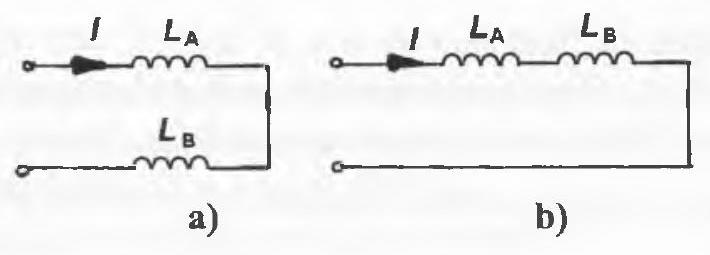
\includegraphics[max width=\textwidth, center]{2025_07_01_5b3ff9fa0d508c8e9f17g-187(1)} Fig. 3.32\\

3.190.* Care dintre afirmațiile următoare referitoare la fenomenul de inducție electromagnetică este falsă?\\ A) dacă o spiră conductoare închisă este rotită în jurul unuia din diametrele sale care este perpendicular pe liniile unui câmp magnetic uniform, constant în timp, în spiră se induce curent electric; B) dacă o spiră de sârmă, închisă, este rotită astfel încât normala la suprafața ei rămâne permanent paralelă cu liniile unui câmp magnetic uniform, constant în timp, în spiră nu apare curent electric indus; C) dacă o spiră de sârmă, închisă, este rotită în jurul unui diametru al ei care este paralel cu liniile unui câmp magnetic uniform, constant în timp, în spiră nu apare curent electric indus; D) dacă o spiră de sârmă, închisă, este translatată într-un câmp magnetic uniform, constant în timp, în spiră apare curent electric indus; E) dacă o spiră de sârmă, închisă, este scoasă dintr-un câmp magnetic uniform, constant în timp, în spiră apare curent electric indus; F) N/A.\\ (Eugen Scarlat)\\

3.191.* O spiră conductoare de rază $R$ este întreruptă printr-un condensator C (Fig. 3.33). Spira este plasată într-un câmp magnetic variabil. Cunoscând viteza de variatie a inductiei magnetice $\frac{\Delta B}{\Delta t}$, sarcina condensatorului este:\\ A) $q=R^{2} C \frac{\Delta B}{\Delta t}$; B) $q=\pi \frac{\Delta B}{\Delta t} C$; C) $q=\pi R^{2} C \frac{\Delta B}{\Delta t}$; D) $q=\pi R^{2} \frac{\Delta B}{\Delta t}$; E) $q=\frac{C}{\pi R^{2}} \frac{\Delta B}{\Delta t}$; F) $q=\frac{C}{\pi R^{2}} \frac{\Delta B}{\Delta t}$.\\ (Gherghe Stanciu)\\ 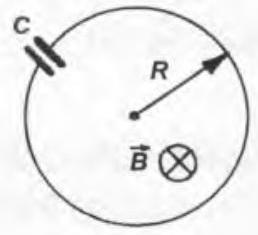
\includegraphics[max width=\textwidth, center]{2025_07_01_5b3ff9fa0d508c8e9f17g-188} Fig. 3.33\\

3.192.* O bobină cu 1000 spire cu aria de $20 \mathrm{~cm}^{2}$ este rotită, dintr-o poziție în care planul spirelor sale este perpendicular pe câmpul magnetic al Pământului, în poziția în care planul este paralel cu câmpul, în $0,02 \mathrm{~s}$. Tensiunea electromotoare medie indusă, dacă inducția câmpului magnetic al Pământului este de $6 \cdot 10^{-5} \mathrm{~T}$ este egală cu:\\ A) $5 \cdot 10^{-3} \mathrm{~V}$; B) $0,15 \mathrm{~V}$; C) $1 \mathrm{~V}$; D) $3 \mathrm{~mV}$; E) $6 \mathrm{~mV}$; F) $0,03 \mathrm{~V}$.\\ (Ionuț Puică)\\

3.193.* Un solenoid de lungime $L$ şi rază $r$ este bobinat uniform cu $N_{1}$ spire. O a doua bobină cu $N_{2}$ spire este aşezată concentric în jurul solenoidului, la mijlocul acestuia. Factorul de proportionalitate între fluxul total prin a doua bobină datorat unui curent prin prima bobină (solenoid) şi valoarea acestui curent (această mărime poartă numele de inductanța mutuală $M$ a celor două bobine) este:\\ A) $\mu_{0} N_{1} \pi r^{2} / N_{2} L$; B) $\mu_{0} N_{1} N_{2} L$; C) $N_{1} N_{2} \pi r^{2} / L$; D) $\mu_{0} N_{1} N_{2} r^{2} / L$; E) $\mu_{0} N_{1} N_{2} \pi r^{2} / L$; F) $\mu_{0} N_{1} N_{2} 2 \pi r$.\\ (Ionuț Puică)\\

3.194.* Printr-o bobină trece un curent $I_{1}=2 \mathrm{~A}$. Intensitatea $I_{2}$ a curentului printr-o altă bobină, cu lungimea de 2 ori mai mare decât prima, celelalte elemente fiind aceleaşi, pentru a produce acelaşi flux magnetic este:\\ A) $1 \mathrm{~A}$; B) $0,5 \mathrm{~A}$; C) $4 \mathrm{~A}$; D) $2 \mathrm{~A}$; E) $5 \mathrm{~A}$; F) $0,5 \mathrm{~A}$.\\ (Marin Cilea)\\

3.195.* O bară conductoare de lungime $l=0,1 \mathrm{~m}$ alunecă cu o viteză $v=1 \mathrm{~m} / \mathrm{s}$ de-a lungul a două bare perfect conductoare, paralele, legate printr-un rezistor de rezistență $R=0,2 \Omega$. Sistemul este plasat într-un câmp magnetic uniform de inducție $B$, perpendicular pe planul barelor. Neglijând frecările, valoarea lui $B$ pentru ca prin bara mobilă să circule un curent de $1 \mathrm{~A}$ este:\\ A) $1 \mathrm{~T}$; B) $2 \mathrm{~T}$; C) $3 \mathrm{~T}$; D) $4 \mathrm{~T}$; E) $5 \mathrm{~T}$; F) $6 \mathrm{~T}$.\\ (Marin Cilea)\\

3.196.* O bară metalică de $2 \mathrm{~m}$ lungime cade paralel cu ea însăşi într-un câmp magnetic orizontal uniform cu inducția de $2 \cdot 10^{-5} \mathrm{~T}$ sub acțiunea greutății. Însă, datorită unei frânări, mişcarea sa devine uniformă, cu viteza de $10 \mathrm{~m} / \mathrm{s}$. Diferența de potential dintre capetele barei este:\\ A) $0,2 \mathrm{mV}$; B) $0,4 \mathrm{mV}$; C) $0,6 \mathrm{mV}$; D) $0,5 \mathrm{mV}$; E) $0,8 \mathrm{mV}$; F) $0,4 \mathrm{~V}$.\\ (Constantin Neguțu)\\

3.197.* Un electron cu o energie cinetică de $10 \mathrm{eV}\left(1 \mathrm{eV}=1,6 \cdot 10^{-19} \mathrm{~J}\right)$ se roteşte într-un câmp magnetic uniform de inducție $B=10^{-4} \mathrm{~T}$. ( $m_{0}=9,1 \cdot 10^{-31} \mathrm{~kg},|e|=1,6 \cdot 10^{-19} \mathrm{C}$ ). Raza traiectoriei şi perioada de rotație au valorile:\\ A) $R=5,3 \mathrm{~cm}, T=3,6 \cdot 10^{-7} \mathrm{~s}$; B) $R=10,7 \mathrm{~cm}, T=3,6 \cdot 10^{-7} \mathrm{~s}$; C) $R=20 \mathrm{~cm}, T=12 \cdot 10^{-6} \mathrm{~s}$; D) $R=15 \mathrm{~cm}, T=1 \mathrm{~s}$; E) $R=11,8 \mathrm{~cm}, T=3 \cdot 10^{-6} \mathrm{~s}$; F) $R=9 \mathrm{~cm}, T=3 \cdot 10^{-9} \mathrm{~s}$.\\ (Constantin Neguțu)\\

3.198.* Alegeți afirmația adevărată:\\ A) Câmpul magnetic al unui solenoid are liniile de câmp deschise; B) Inducția câmpului magnetic produs de un curent electric scade dacă intensitatea curentului creşte; C) La distanţă $r$ de un conductor rectiliniu, infinit, parcurs de un curent de intensitate $I$, inducţia magnetică este $B=\frac{\mu I}{2 r}$; D) Asupra unui conductor parcurs de un curent electric şi aşezat perpendicular pe liniile unui câmp magnetic exterior nu se exercită o forță electromagnetică; E) În centrul unei spire de rază $r$, parcursă de curentul de intensitate $I$, inducția magnetică este $B=\frac{\mu I}{2 \pi r}$; F) Pe axa unui solenoid subțire inducția magnetică este $B=\frac{\mu N I}{l}$.\\ (Constantin Neguțu)\\

3.199.* Forța exercitată asupra unui conductor având lungimea egalǎ cu $2 \mathrm{~cm}$ , parcurs de un curent de intensitate $I=10 \mathrm{~A}$ într-un câmp magnetic uniform de inducție $B=1 \mathrm{mT}$ atunci când conductorul este orientat: a) perpendicular; b) sub un unghi $\alpha=60^{\circ}$ față de câmp are valorile:\\ A) $4 \cdot 10^{-2} \mathrm{~N}, 2 \cdot 10^{-2} \mathrm{~N}$; B) $2 \cdot 10^{-2} \mathrm{~N}, 10^{-2} \mathrm{~N}$; C) $8 \cdot 10^{-2} \mathrm{~N}, 4 \cdot 10^{-2} \mathrm{~N}$; D) $4 \cdot 10^{-2} \mathrm{~N}, \sqrt{3} \cdot 10^{-2} \mathrm{~N}$; E) $2 \cdot 10^{-4} \mathrm{~N}, \sqrt{3} \cdot 10^{-4} \mathrm{~N}$; F) $\sqrt{3} \cdot 10^{-2} \mathrm{~N}, 2 \cdot 10^{-2} \mathrm{~N}$.\\ (Daniela Buzatu)\\

3.200.* O spiră circulară cu raza $r=4 \mathrm{~cm}$ şi rezistența $R=0,04 \Omega$ este plasată într-un câmp magnetic uniform de inducție $B=0,2 \mathrm{~T}$. Poziția inițială a spirei este paralelă cu liniile de câmp. Sarcina electrică ce trece prin spiră la rotirea ei cu unghiul $\alpha=30^{\circ}$ este:\\ A) $4 \pi \mathrm{mC}$; B) $\pi \mathrm{mC}$; C) $16 \pi \mathrm{mC}$; D) $2 \pi \mathrm{mC}$; E) $0,04 \pi \mathrm{mC}$; F) $0,1 \pi \mathrm{mC}$.\\ (Daniela Buzatu)\\

3.201.* Prin anularea uniformă a inducției câmpului magnetic uniform $B$, în intervalul $\Delta t=0,1 \mathrm{~s}$, se induce într-o bobină cu $N=1500$ spire, tensiunea electromotoare $e=15 \mathrm{~V}$. Fluxul magnetic $\Phi$ printr-o spiră a bobinei este egal cu:\\ A) $15 \cdot 10^{-3} \mathrm{~Wb}$; B) $0,1 \cdot 10^{-3} \mathrm{~Wb}$; C) $1 \cdot 10^{-3} \mathrm{~Wb}$; D) $1,5 \cdot 10^{-3} \mathrm{~Wb}$; E) $0,01 \cdot 10^{-3} \mathrm{~Wb}$; F) $0,15 \cdot 10^{-3} \mathrm{~Wb}$.\\ (Daniela Buzatu)\\

3.202.* Un ion bivalent se mişcă cu viteza $v=160 \mathrm{~km} / \mathrm{s}$ într-un câmp magnetic omogen de inducție $B=0,01 \mathrm{~T}$. Masa ionului, dacǎ el descrie un cerc de rază $R=10 \mathrm{~cm}$, este egală $\mathrm{cu}\left(e=1,6 \cdot 10^{-19} \mathrm{C}\right)$ :\\ A) $10^{-27} \mathrm{~kg}$; B) $0,5 \cdot 10^{-27} \mathrm{~kg}$; C) $2 \cdot 10^{-27} \mathrm{~kg}$; D) $4 \cdot 10^{-27} \mathrm{~kg}$; E) $16 \cdot 10^{-27} \mathrm{~kg}$; F) $8 \cdot 10^{-27} \mathrm{~kg}$.\\ (Daniela Buzatu)\\

3.203. Un bec cu tensiunea nominală $U=6 \mathrm{~V}$ şi puterea nominală $P=2 \mathrm{~W}$ trebuie alimentat de la o sursă de cc. cu t.e.m. $E=12 \mathrm{~V}$ şi rezistența internă neglijabilă. Să se calculeze rezistența rezistorului ce trebuie montat în circuit pentru ca becul să funcționeze normal.\\ A) $18 \Omega$; B) $28 \Omega$; C) $14 \Omega$; D) $1,8 \Omega$; E) $10 \Omega$; F) $12 \Omega$.\\ (Ioana Ivaşcu)\\

3.204. O baterie debitează pe un rezistor de rezistență $R_{1}=5 \Omega$ un curent de intensitate $I_{1}=0,8 \mathrm{~A}$. Inlocuind rezistorul cu un altul de rezistență $R_{2}=6 \Omega$ intensitatea curentului electric devine $I_{1}=0,6 \mathrm{~A}$. T.e.m. a bateriei are valoarea:\\ A) $2,4 \mathrm{~V}$; B) $2,6 \mathrm{~V}$; C) $1,4 \mathrm{~V}$; D) $1,8 \mathrm{~V}$; E) $1 \mathrm{~V}$; F) $1,2 \mathrm{~V}$.\\ (Ioana Ivaşcu)\\

3.205.* Un cadru metalic rigid, fară posibilități de rotire, ce delimitează o suprafață de arie $S$ se află într-un câmp magnetic uniform de inducție $B=a+b t$ ($T$), cu $a$ şi $b$ constante. T.e.m. indusă în cadru în unitatea de timp este:\\ A) $S b$; B) $S a$; C) $S a b$; D) $S b^{2}$; E) $S a^{2}$; F) $0 \mathrm{~T}$.\\ (Ioana Ivaşcu)\\

3.206. O baterie având t.e.m. $E$ şi rezistența internă $r$ dezvoltă pe un rezistor aceeaşi putere $P$, pentru două valori ale rezistenței acestuia $R_{1}$ şi $R_{2}$. Intensitatea curentului de scurtcircuit a sursei este:\\ A) $\frac{E}{\sqrt{R_{2}}} R_{1}$; B) $\frac{E^{2}}{\sqrt{R_{1} R_{2}}}$; C) $\frac{2 E}{\sqrt{R_{1} R_{2}}}$; D) $\frac{E}{\sqrt{R_{1} R_{2}}}$; E) $\frac{E}{\sqrt{2 R_{1} R_{2}}}$; F) $\frac{E}{\sqrt{R_{1}}} R_{1}$.\\ (Ioana Ivaşcu)\\

3.207. Cunoscând intensitatea curentului de scurtcircuit $I_{\mathrm{s}}$ a unei baterii, să se determine randamentul circuitului electric alimentat de această baterie, ştiind că intensitatea curentului electric prin circuit este $I$.\\ A) $\eta=1-\frac{I}{I_{s}}$; B) $\eta=1-\frac{I_{s}}{I}$; C) $\eta=1+\frac{I}{I_{s}}$; D) $\eta=\frac{I}{I_{s}}-1$; E) $\eta=1-\frac{2 I}{I_{s}}$; F) $\eta=1-\frac{I}{2 I_{s}}$.\\ (Ioana Ivaşcu)\\

3.208.* Un ion pozitiv cu sarcina $q$ intră într-un câmp magnetic având viteza $v$, după o direcție care face unghiul $\alpha$ cu direcția liniilor de câmp. Raza elicoidei descrise de mişcarea ionului este:\\ A) $\frac{m v \sin \alpha}{q B}$; B) $\frac{m v \sin \alpha}{2 q B}$; C) $\frac{m v^{2} \sin \alpha}{q B}$; D) $\frac{m v \cos \alpha}{q B}$; E) $\frac{m v \cos \alpha}{2 q B}$; F) $\frac{2 m v \sin \alpha}{q B}$.\\ (Ioana Ivaşcu)\\

3.209. Legând un rezistor de rezistentă $R$ la un generator de curent continuu tensiunea la borne este $U$. Înlocuind rezistorul cu un altul având rezistența de 4 ori mai mare tensiunea la borne creşte cu $n \%$. Să se determine t.e.m. a generatorului.\\ A) $E=\frac{3 U(n+1)}{3-n}$; B) $E=\frac{3 U(n-1)}{3-n}$; C) $E=\frac{4 U(n+1)}{3-n}$; D) $E=\frac{3 U(n+1)}{3-2 n}$; E) $E=\frac{U(n+1)}{3-n}$; F) $E=\frac{U(3 n+1)}{3-n}$.\\ (Ioana Ivaşcu)\\

%% End %%